%%**************************************************************************************************
%%
%% File Name : PhysNote_EM_2nd.tex
%% 説明      : 電磁気学をマクスウェル方程式を基礎(前提)にして,学習する.
%%
%%**************************************************************************************************
%===================================================================================================
%  Chapter : 電磁気学の再構築
%  説明    : これまでは,マクスウェル方程式を導くように電磁気学を学習してきた.しかし,現在の電磁気学
%            の体系はマクスウェル方程式を基礎にした記述である.そこで,今までの電磁気学のイメージを取
%            り払うよう,注意を呼びかける.
%===================================================================================================
\chapter{電磁気学の再構築}
%   %-----------------------------------------------------------------------------------------------
%   %  Input
%   %    File Name : PhysNote_EM_2nd_MsgFirst.tex
%   %    説明      : マクスウェル方程式を前提に話を進める上での,心構え.
%   %-----------------------------------------------------------------------------------------------
        %===================================================================================================
%  Chapter : 電磁気学の再構築
%  説明    : これまでは,マクスウェル方程式を導くように電磁気学を学習してきた.しかし,現在の電磁気学
%            の体系はマクスウェル方程式を基礎にした記述である.そこで,今までの電磁気学のイメージを取
%            り払うよう,注意を呼びかける.
%===================================================================================================
%   %==========================================================================
%   %  Section
%   %==========================================================================
    \section{もう一度はじめから}
%   %==========================================================================
%   %  SubSection
%   %==========================================================================
        \subsection{帰納的な考え方}
        これまでは,マクスウェル方程式を導くように電磁気学を学習してきた.
        すでに知られている実験事実を基に,物理法則を導出するという考え方を,
        \textbf{帰納的} な考え方であるという.とにかく,今知られている事実
        から,どんなことが言えるかを,直感をもとにして探し出すのである.
        このような帰納的な考え方は,新しい概念をい知識として吸収するのに,
        有効である.

        例えば,小学校や中学校における,算数や数学の授業では,新しい概念
        を教わるとき,必ず具体的な例を見た後に,「これは一般的に成り立つ」
        というように教わるはずである.このような学習方法は確かに分かりやすい
        が,論理的であるとは言えない.何しろ直感をもとにして,説明をしている
        のだから,仕方がないのであるが,ものごとをきちんと整理して把握するの
        には,この方法は不適切である.そこで,次の段階として,帰納的に導いた
        事柄(ここではマクスウェル方程式)をもとにして,理論を再構成する作業
        が必要になってくる.
            \begin{figure}[hbt]
                \begin{center}
                    \includegraphicsdefault{KinouTekiSuiron.pdf}
                    \caption{帰納的推論}
                    \label{fig:KinouTekiSuiron}
                \end{center}
            \end{figure}



%   %==========================================================================
%   %  SubSection
%   %==========================================================================
        \subsection{演繹的な考え方}
        何かの理論を構築する際に,あるいくつかの約束事を,納得するか否かに関わ
        らずに,強制的に認めさせる.そして,この強制的に与えられた約束事を元に
        して,理論を構築する.もちろん論理的に作らないといけない.最初の約束事
        さえ認めれば,その後は,論理的推論で導き出せるように,理論を構成するの
        である.このような考え方を,\textbf{演繹的} な考え方であるという.

        演繹的な考え方は,理論を論理的に構築する際に,とても役に立つ.ただ,問
        題なのは,最初に与える約束事が認められない,あるいは疑わしさを感じ
        る場合である
            \footnote{
                集合論などの,選択公理などは,その最も有名なものではなかろうか.
            }.
        この場合,論理の最も基礎の部分に不安があるため,いくら論理的に理論を構
        築したところで,この理論の正当性も怪しまれてしまう.なので,その最も基
        礎となる約束事は,できるだけ確かな事実を採用すべきだ.それには,
        帰納的な考え方が適している.帰納的に導きだされた結果は,直感的になじみ
        やすいからである.
            \begin{figure}[hbt]
                \begin{center}
                    \includegraphicslarge{EnnekiTekiSuironn.pdf}
                    \caption{演繹的推論}
                    \label{fig:EnnekiTekiSuironn}
                \end{center}
            \end{figure}


%   %==========================================================================
%   %  SubSection
%   %==========================================================================
        \subsection{“帰納”から“演繹”へ}
        物事を論理的に構成しようとするとき,まず土台
            \footnote{
                土台:有無を言わさず,認めさせる,最初の約束事.
            }
        が必要である.その土台は,おおよそ間違いを含まず,正当性が高いものであ
        る必要がある.このような理論の土台を得るには,まず帰納的に考えるとよい.
        帰納的に考えるとは,実験をして,その結果を説明できるような法則を考える
        ということである.これには,多くの実験を行う必要があることだろう.何度も
        何度も,実験を行う.そうして,いろいろな実験結果が揃う.そして,それらを
        説明する理論も,同じくらい多くなっていることだろう.そうした段階で,少々
        立ち止まって,考えてみる.今度は,頭と鉛筆と紙で考えるのである.多くの
        実験で,多くの理論が創りだされた.しかし,この多くの理論には,いくつかの
        共通点が存在するはずであると考え,その共通点を探し出すのだ.いくら考えて
        も共通点がないかもしれないが,こればかりはやってみなければわからない.
        運良く,それらの共通点が明らかになった場合には,より簡潔な理論を作り出せ
        る可能性がある.そしたら,共通点を法則として捉え直し,演繹的な理論構築
        の土台にするのだ.たくさんの実験から得られた土台(法則)だから,それだけ
        に説得力があり,正当性の保証も大きい.

        帰納的な考え方から,演繹的な考え方に思考を切り替えるのには,それ相応の困
        難があることと思う.しかし,理論を組み上げる上で,この考え方の切り替えは
        非常に重要なことである.以下では,今までに帰納的に導いてきたマクスウェル
        方程式を土台とし,演繹的な理論構築の基礎に置き,電磁気学的な現象をとらえ
        なおしていくことにしよう.

%       %======================================================================
%       %  SubSection
%       %======================================================================
        \subsection{演繹的な電磁気理論の組み立て方}
        電磁気理論を再構築するに当たって,まず,その構成の手順を示しておくと,
        後の話の流れが把握しやすいだろう.

        構築の仕方は色いろあるだろうが,ここでは,太田浩一によって著された
        \cite{bib:refbook_em_5}の構成で学習を進めていくことにする.以下に,
        その概略を書いておこう.

        まず,力学との接点として,クーロンの法則を採用する.そして,特殊相対性
        理論の学習で導いたローレンツ変換
            \footnote{
                ローレンツ力ではないよ.
            }
        をクーロン力に対して,適用する.その適用結果を式変形すると,
        電磁場のローレンツ力と同じ形の力が導出される.これは,もちろん,
        ローレンツ力とみなすことができる.このローレンツ力をもとに,
        電場と磁束密度を定義する.最後に,マクスウェル方程式を,電場と磁束密度
        が満たす条件として,付け加える.


%   %-----------------------------------------------------------------------------------------------
%   %  Input
%   %    File Name : PhysNote_EM_2nd_ReMkTheory.tex
%   %    説明      : 電磁気学を再構築する.
%   %-----------------------------------------------------------------------------------------------
        %===================================================================================================
%  Chapter : 電磁気学の再構築
%  説明    : これまでは,マクスウェル方程式を導くように電磁気学を学習してきた.しかし,現在の電磁気学
%            の体系はマクスウェル方程式を基礎にした記述である.そこで,今までの電磁気学のイメージを取
%            り払うよう,注意を呼びかける.
%   %==========================================================================
%   %  Section
%   %==========================================================================
    \section{クーロンの法則}
        クーロンの法則は,電気の性質を示す最も基礎的な法則である.
        電気の性質をもつ物体を,\textbf{電荷} とよぶ
            \footnote{
                「電荷」と書いたとき,その物体の他の性質(大きさ,重さ等)は
                無視して,電気的性質のみに着目する.
            }.
        \begin{myshadebox}{クーロンの法則}
            クローンの法則が示す電気的性質とは,以下の通り.
            \begin{itemize}
                \item   電気には,"正(Plus)"と"負(Minus)"の2種類が存在する
                \item   2つの電荷が異種(正と負)であれば,各々の電荷
                      は互いに引き合う向きに力を受ける
                \item   2つの電荷が同種(正と正/負と負)であれば,各々の電荷
                      は互いに反発し合う向きに力を受ける
                \item   2つの電荷が受ける力の大きさは等しく,力の向きは互いに逆向きである
                \item   2つの電荷が受ける力の大きさは,2つの電荷の電気量の積に比例する
                \item   2つの電荷が受ける力の大きさは,2つの電荷の距離の2乗に反比例する
            \end{itemize}
        \end{myshadebox}
        \begin{myshadebox}{クーロン力}
            ある空間に2つの電荷 $q_{1}$,$q_{2}$ が,それぞれ
            位置 $\br_{1}$,$\br_{2}$ に
            存在するとき,この2つの電荷には,次式で
            表されるような力が作用する.この力のこと
            を \textbf{クーロン力} という.

            電荷 $q_{1}$ に対しては,
               \begin{align}
                   \bF_{12} =
                       \frac{1}{4\pi\varepsilon_{0}} \frac{q_{1}q_{2}}{r^{2}}
                           \frac{\br_{1} - \br_{2}}{|\br_{1} - \br_{2}|}
               \end{align}
            という力が働く.

            ここに,$\varepsilon_{0}$ は真空の誘電率である.
        \end{myshadebox}

        \begin{figure}[hbt]
            \begin{tabular}{cc}
                \begin{minipage}{0.5\hsize}
                    \begin{center}
                        \includegraphicsdouble{coulombs_low1.pdf}

                        (A)
                    \end{center}
                \end{minipage}
                \begin{minipage}{0.5\hsize}
                    \begin{center}
                        \includegraphicsdouble{coulombs_low2.pdf}

                        (B)
                    \end{center}
                \end{minipage}
            \end{tabular}
                        \caption{クーロン力((図\ref{fig:coulombs_low}) 再揚)}
        \end{figure}


%   %==========================================================================
%   %  Section
%   %==========================================================================
    \section{ローレンツ変換}

%   %==========================================================================
%   %  Section
%   %==========================================================================
    \section{電場と磁束密度の定義}

%   %==========================================================================
%   %  Section
%   %==========================================================================
    \section{マクスウェル方程式}
%   %==========================================================================
%   %  SubSection
%   %==========================================================================
        \subsection{ファラデーの電磁誘導の法則}

%   %==========================================================================
%   %  SubSection
%   %==========================================================================
        \subsection{アンペール$=$マクスウェルの法則}

%   %==========================================================================
%   %  SubSection
%   %==========================================================================
        \subsection{電場に対するガウスの法則}

%   %==========================================================================
%   %  SubSection
%   %==========================================================================
        \subsection{磁束密度に対するガウスの法則}

%   %==========================================================================
%   %  Section
%   %==========================================================================
    \section{電荷保存の法則}
    \begin{mysmallsec}{マクスウェル方程式は,その内部に電荷保存則を含んでいる}
        マクスウェルの法則(マクスウェル方程式)は,その内部に,電荷保存則を含んでいる.
        つまり,マクスウェル方程式から,電荷保存則を導けるのである.
        このノートでは前に,電荷保存の法則を仮定して マクスウェル方程式を
        導いたわけだが,今回はマクスウェル方程式を仮定して,電荷保存の法則を導出する
            \footnote{
                電荷保存則を仮定して,マクスウェル方程式を見つけ出したのだから,
                その内部に電荷保存則を含んでいることは,当然である.
            }.
        今日では,マクスウェル方程式を仮定して電磁気現象を説明するという立場があたりまえになっている.
        このようなことから,電荷保存の法則は法則ではなく,
        定理(法則から導かれる現象)として捉えるべきだ.
    \end{mysmallsec}

    \begin{mysmallsec}{導出}
        アンペール$=$マクスウェルの法則の両辺に,$\ddiv$ をとると
        \footnote{
            電流や変位電流の発散が電荷密度の移動であると表現したいので,
            このような操作をする.
        },
        \begin{align*}
            \ddiv\mu_{0}\left( \bi + \varepsilon_{0}\frac{\rd \bE}{\rd t} \right)
            &=\ddiv\drot\bB \\
            \Leftrightarrow
                \mu_{0}\left(\ddiv\bi+ \varepsilon_{0}\frac{\rd (\ddiv\bE)}{\rd t} \right)
            &=\ddiv\drot\bB
        \end{align*}
        である.ここで, $\ddiv$ は空間に関する作用であり, $\rd/\rd t$ は時間に対する作用であるから,
        両者は可換である.
        これに加えて,電場に対するガウスの法則 $\ddiv\bE=\rho/\varepsilon_{0}$ から,
        \begin{align*}
                \mu_{0}\left(\ddiv\bi+\frac{\rd }{\rd t}\rho\right)=\mathrm{div\,rot}\bB
        \end{align*}
        である.最後に,ベクトル解析の恒等式;任意の $\bM$ に対して,$\mathrm{div\,rot}\bM:= 0$ で
        あることを考慮すれば,
        \begin{align}
            \ddiv\bi+ \frac{\rd }{\rd t} \rho =0
        \end{align}
        を得る.これは電荷保存の法則を表現する式である.
    \end{mysmallsec}


%   %==========================================================================
%   %  Section
%   %==========================================================================
    \section{マクスウェル方程式の解}
    \begin{mysmallsec}{変数の個数と,方程式の個数が一致しない}
        マクスウェル方程式をなす4つの方程式は,電場と磁束密度を変数とする方程式である.
        電場と磁束密度はそれぞれ3つの方向成分をもっている.従って,マクスウェル方程式
        によって決定されるべき未知関数は,$3\times2$ で6個である.
        具体的には,$E_{x}(\br,\,t)$,$E_{y}(\br,\,t)$,$E_{z}(\br,\,t)$,
        $B_{x}(\br,\,t)$,$B_{y}(\br,\,t)$,$B_{z}(\br,\,t)$ である.

        ところで,マクスウェル方程式を見てみると,これらは成分で見れば8この方程式で
        あると言える.具体的にいえば,電磁誘導の法則で3つ,アンペール$=$マクスウェルの法則で3つ,
        電場に対するガウスの法則で1つ,磁束密度に対するガウスの法則で1つの
        合計 $3+3+1+1$ で8個となる
            \footnote{
                電磁誘導の法則やアンペールの法則は,ベクトルで記述されている方程式で
                あるから,その方程式には3つの方向成分($x$ 成分,$y$ 成分,$z$ 成分)
                をもっている.従って,法則の各々に,未知関数が3ずつ含まれているので
                ある.また,2つのガウスの法則はスカラー方程式であるので,未知関数は
                各々の法則で1つである.
            }.

        つまり,\textbf{方程式の個数の方が変数の個数よりも
        2つ多いということになり,矛盾なく解が求まるかどうか}といった
        疑問が生じるのである.結論から先にいえば,矛盾なく解が求まるのである.
        というのも,電場に対するガウスの法則が電場の初期条件を与え,
        磁束密度に対するガウスの法則が磁束密度の初期条件を与える式と
        考えられるのである.
    \end{mysmallsec}

    \begin{mysmallsec}{数式により,確認}
        以上のことを数式で表現すれば次のようになる.

        まず,ファラデーの電磁誘導の法則の両辺に $\ddiv$ をとる.
        \begin{align}
            \mathrm{div\,rot\,} \bE
            &=\mathrm{div\,}\left( -\frac{\rd \bB}{\rd t}\right) \notag \\
            \Leftrightarrow \quad
            \mathrm{div\,rot\,} \bE
            &=-\frac{\rd \left(\mathrm{div\,}\bB\right)}{\rd t}
        \end{align}

        さて,ベクトル解析の公式から,任意のベクトルを $\bC$ として,
        $\mathrm{div\,rot\,} \bC:=0$ が成立しているので,上式の右辺は
        恒等的に0となって,結局,
        \begin{align}
            -\frac{\rd \left(\mathrm{div\,}\bB\right)}{\rd t} =0
        \end{align}
        となる.磁束密度の初期条件として,磁束密度に対するガウスの法則を使えば,
        電磁場が変動してもファラデーの法則は自動的に成り立つのである.

        また電場についても,アンペール$=$マクスウェルの法則の両辺に $\ddiv$ をとれば,
        \begin{align}
            \mathrm{div\,}\left(\mathrm{rot\,}\bB\right)
            &=
            \mathrm{div\,}\mu_{0}
            \left(\bi+
                \varepsilon_{0}\frac{\rd \bE}{\rd t}
            \right) \notag \\
            \Leftrightarrow \quad
            \mathrm{div\,rot\,}\bB
            &=
            \mu_{0}\mathrm{div\,}\bi+
            \varepsilon_{0}\mu_{0}\frac{\rd (\mathrm{div\,}\bE)}{\rd t}
        \end{align}
        である.

        さて,ベクトル解析の公式から,任意のベクトルを $\bC$ として,
        $\mathrm{div\,rot\,} \bC:=0$ が成立しているので,上式の右辺は
        恒等的に0となって,
        \begin{align}
            \mathrm{div\,}\bi+
            \varepsilon_{0}\frac{\rd (\mathrm{div\,}\bE)}{\rd t}
            &=
            0
        \end{align}
        と書ける.ここで,
        電荷保存の法則より,$\ddiv\bi=-\rd/\rd t\rho$ を上式考慮すると,
        \begin{align}\label{eq:Gauss_first}
            \frac{\rd }{\rd t}\rho
            -\varepsilon_{0}\frac{\rd (\mathrm{div\,}\bE)}{\rd t}
            &=
            0 \notag \\
            \Leftrightarrow \quad
            \frac{\rd }{\rd t}
            \left(\rho
                -\varepsilon_{0}\mathrm{div\,}\bE
            \right)
            &=
            0
        \end{align}
        を得る.電場に対するガウスの法則を電場の初期条件として考えるならば,
        アンペール$=$マクスウェルの法則は,電場がこの後時間変化しても,成立する.

        つまり,上式(\ref{eq:Gauss_first})を時間積分して,
            \begin{equation*}
                \rho - \varepsilon_{0} \ddiv \bE = C\,,\quad \mbox{(Cは積分定数)}
            \end{equation*}
        だが,初期条件がガウスの法則によって書かれるものであるとするなら,定数 $C=0$ であり,
            \begin{equation*}
                \rho - \varepsilon_{0} \ddiv \bE =0
            \end{equation*}
            \begin{equation*}
                 \ddiv \bE =\frac{\rho}{\varepsilon_{0}}
            \end{equation*}
        さて以上によって,マクスウェル方程式を矛盾することなく解くことができるということが
        示された.
    \end{mysmallsec}


%===================================================================================================
%  Chapter : 真空中の電磁波
%  説明    : マクスウェル方程式をもとに,真空中の電磁波の波動方程式を導出し,
%            また,電磁波の性質について考える
%===================================================================================================
\chapter{真空中の電磁波}
%   %-----------------------------------------------------------------------------------------------
%   %  Input
%   %    File Name : PhysNote_EM_2nd_RadioWave.tex
%   %    説明      : 電磁波の波動方程式を導き,その性質も学習する.
%   %-----------------------------------------------------------------------------------------------
        %===================================================================================================
%  Chapter : 真空中の電磁波
%  説明    : マクスウェル方程式をもとに,真空中の電磁波の波動方程式を導出し,
%            また,電磁波の性質について考える
%===================================================================================================
%   %==========================================================================
%   %  SubSection
%   %==========================================================================
    \section{波動方程式}
        \begin{mycomment}
            最初に,波動方程式について,簡単にまとめておこう
            \footnote{
                詳細は,微分方程式の教科書を参照すること.
            }.
        \end{mycomment}

    \subsection{波動関数}
        波動方程式の解は \textbf{波動関数} である.波動関数とは,実際の現象として
        起きている \textbf{波} もしくは \textbf{波動} を,数学的な関数として抽象化
        したものである.これにより,波という現象を数学的に解析できるようになる.
        波動方程式を考える前に,\textbf{波} もしくは \textbf{波動} について調べておく
        必要がある.


    \subsection{波動方程式の導出}
        2つの独立変数 $x$,$t$ をもつ関数 $K(x,\,t)$ に関する \textbf{波動方程式} とは,
        以下の偏微分方程式のことを言う.
        \begin{align}
            \frac{{\rd}^{2} K}{{\rd t}^{2}}  = a \frac{{\rd}^{2}K}{{\rd x}}.
        \end{align}

%   %==========================================================================
%   %  Section
%   %==========================================================================
    \section{真空中のマクスウェル方程式}
        \begin{mycomment}
        前章で確認した 微分形のマクスウェル方程式 を用いて,電磁波について考える.
        まず,電場の波動方程式 と 磁束密度の波動方程式 を
        別々に確認する.そして,ファラデーの電磁誘導の法則 と 電場に対する
        ガウスの法則から,それら2つの波動方程式の関係を考える.
        \end{mycomment}

%   %==========================================================================
%   %  SubSection
%   %==========================================================================
    \subsection{マクスウェル方程式の確認}
        マクスウェルの方程式を書き下しておく.
        \begin{align}
            \drot \bE
            &=
            -\frac{\rd \bB}{\rd t}\\
            \drot\bB
            &=
            \mu_{0}\left(\bi+
                \varepsilon_{0}\frac{\rd \bE}{\rd t}
            \right)\\
            \ddiv\bE
            &=\frac{\rho}{\varepsilon_{0}}\\
            \ddiv\bB
            &=
            0\\
        \end{align}

%   %==========================================================================
%   %  SubSection
%   %==========================================================================
    \subsection{真空中であることの仮定}
        電磁波を考えるにあたって 話を簡単にするために,以下の仮定を設ける.これは
        真空中の電磁波を考えることによる要請である.
        \begin{enumerate}
        \item 電荷密度 $\rho$ の分布はないものとする.
                                \begin{align}
                                \rho
                                =0
                                \end{align}
        \item 電流密度 $\bi$ の分布はないものとする.
                                \begin{align}
                                \bi
                                =0
                                \end{align}
        \end{enumerate}




%   %==========================================================================
%   %  SubSection
%   %==========================================================================
    \subsection{電場の波動方程式}
            ファラデーの電磁誘導
            の法則 $\drot \bE=-\rd \bB/\rd t$ の
            両辺に $\drot$ をとる.
                                    \begin{align}
                                    \mathrm{rot\,rot} \bE
                                    &=
                                    -\drot\frac{\rd \bB}{\rd t}
                                    \end{align}
            ここで,ベクトル解析の公式 $\mathrm{rot\, rot}=\mathrm{grad\, div}-\Delta$ を適用する
                \footnote{
                    ここに,
                        \begin{align*}
                            \Delta:=
                            \mathrm{div\, grad}=
                            \frac{\rd^{2}}{\rd x^{2}}+
                            \frac{\rd^{2}}{\rd y^{2}}+
                            \frac{\rd^{2}}{\rd z^{2}}
                        \end{align*}
                    である.
                }.
            すると,
            \begin{align}\label{denjiha1}
                \mathrm{grad\, div}\,\bE-\Delta\,\bE
                &=
                -\drot\frac{\rd \bB}{\rd t}
            \end{align}
            となる.この式の右辺第1項の $\mathrm{grad\, div}\,\bE$ に注目する.
            電場に対するガウスの法則は,仮定の $\rho=0$ によって,
            \begin{align*}
                \ddiv\bE
                =\frac{1}{\varepsilon_{0}}\rho
                =0
            \end{align*}
            である.従って,$\dgrad0=0$ となって,式(\ref{denjiha1})は
            \begin{align}
                \Delta\,\bE
                &=
                \drot\frac{\rd \bB}{\rd t}
            \end{align}
            と計算される.回転 $\drot$ と時間微分 $\rd/\rd t$ は可換であるから
            \begin{align}\label{denjiha2}
                \Delta\,\bE
                &=
                \frac{\rd (\drot\bB)}{\rd t}
            \end{align}

            ところで,左辺の $\drot\bB$ は アンペール$=$マクスウェルの法則 から
            \begin{align*}
                \drot\bB = \mu_{0}\varepsilon_{0}
                \frac{\rd \bE}{\rd t}
            \end{align*}
            である.ここで,仮定により $\bi=0$ を考慮した.
            これを,式(\ref{denjiha2})に代入して,
            \begin{align}
                \Delta\,\bE &=
                \frac{\rd }{\rd t}\left(\mu_{0}\varepsilon_{0}
                \frac{\rd \bE}{\rd t}\right)\notag \\
                \Leftrightarrow
                \Delta\,\bE
                &=
                \mu_{0}\varepsilon_{0}
                \frac{\rd^{2} \bE}{\rd t^{2}}
            \end{align}
            である.この式を以下のように変形する.
            \begin{align}\label{denjiha3}
                \left(\Delta-\mu_{0}\varepsilon_{0}
                \frac{\rd^{2}}{\rd t^{2}}\right)\bE
                &=0
            \end{align}
            この式は波動方程式と同型である.従って,電場は波動として伝わることを意味する.

            電場の波の位相速度を考える.
            そのために,速度 $\bv$ の位相速度をもつ波動の方程式 $\textit{\textbf{K}}(\br,t)$ を
            書き下す.
            \begin{align}\label{denjiha4}
                \left(\Delta-\frac{1}{v^{2}}
                \frac{\rd^{2}}{\rd t^{2}}\right)\textit{\textbf{K}}
                &=0
            \end{align}
            この式(\ref{denjiha3})と式(\ref{denjiha4})とを見比べてみると,電場の波動方程式の位相速度は
            \begin{align}
                \frac{1}{v^{2}}=\mu_{0}\varepsilon_{0} \notag \\
                \Leftrightarrow
                v=\frac{1}{\sqrt{\mu_{0}\varepsilon_{0}}}
            \end{align}
            である.

            速度を具体的に計算してみるよう.まず,以下の定数は既知である.
            \begin{align*}
                \varepsilon_{0} &= \frac{1}{36\pi\times 10^{9}}\, \mathrm{[F/m]}, \\
                \mu_{0}         &= \frac{4\pi}{ 10^{7}}\, \mathrm{[H/m]}.
            \end{align*}
            これを先の位相速度の式に代入して計算すると,
            \begin{align}
                \frac{1}{\sqrt{\mu_{0}\varepsilon_{0}}}
                &= \frac{1}{\sqrt{\frac{1}{36\pi\times 10^{9}}\,\mathrm{[F/m]} \cdot \frac{4\pi}{ 10^{7}}\,\mathrm{[H/m]}}} \notag \\
                &= 3\times 10^{8} \mathrm{[m/s]}
            \end{align}
            となって,これは光速にかなり近い値である

            この値の妥当性は,ヘルツらの実験により,光速と同等であることが確認された.
            そこで,改めて光速を $c$ と表すことにする
                \footnote{
                    実際は,光速を実験的に測定し,その値に基づいて,$\varepsilon_{0}$ の値が決められている.
                    $\mu_{0}=4\pi \times 10^{-7}$ と定義されているので(電流の定義の項目を参照),
                    光速 $c$ を測り, $c=1/\sqrt{\varepsilon_{0} \mu_{0}}$ の関係から $\varepsilon_{0}$ を計算できる.
                }.
            \begin{align}
                c:=\frac{1}{\sqrt{\varepsilon_{0}\mu_{0}}}\cong 3\times 10^{8} \,\, \mathrm{[m/s]}
            \end{align}

            光速 $c=1/\sqrt{\varepsilon_{0} \mu_{0}}$ を用いて,電場 $\bE$ の波動方程式を表せば,
            \begin{align}
                \left(\Delta-\frac{1}{c^{2}}
                \frac{\rd^{2}}{\rd t^{2}}\right)\bE
                &=0
            \end{align}
            である.

             先ほどは次元の具体的な計算をして指定なかった.次元が速度になることをここで確かめておこう.
             確かめたい次元は
                \[
                    \frac{1}{\sqrt{\mathrm{[F/m]} \mathrm{[H/m]}}} = \mathrm{[m/s]}
                \]
            となることである.次元の括弧を書くのは面倒なので,この計算では省略して記述する.
            まずは,以下のようになることは,簡単にわかる.
                \[
                    \frac{1}{\sqrt{\mathrm{(F/m)} \cdot \mathrm{(H/m)}}} = \frac{1}{\sqrt{\mathrm{FH}/\mathrm{m}^{2}}}.
                \]
            次に $\mathrm{FH}$ の計算を行いたいが,おそらく単位の定義も忘れているだろうから,定義に戻って計算しよう.
            [F]は静電容量の単位で,単位電圧1[V]あたりにためることのできる電荷量[C]$=$[A$\cdot$s]で定義される.
                \[
                    \mathrm{F} := \frac{\mathrm{A}\cdot\mathrm{s}}{\mathrm{V}}.
                \]
            [H]はインダクタンスの単位で,単位時間1[s]の間に1[A]の電流が流れる場合に,
            1[V]の電圧が生じる回路のインダクタンスとして定義される.
                \[
                    \mathrm{H} := \frac{\mathrm{V}}{\mathrm{A/s}} = \frac{\mathrm{V}\cdot\mathrm{s}}{\mathrm{A}}.
                \]
            だから,
                \[
                    \mathrm{F}\cdot\mathrm{H} = \mathrm{s}^{2}.
                \]
            要するに,
                \[
                    \frac{1}{\sqrt{\mathrm{F/m} \mathrm{H/m}}}  = \frac{1}{\sqrt{\mathrm{s}^{2}/\mathrm{m}^{2}}}
                                                                = \frac{1}{\mathrm{s}/\mathrm{m}}
                                                                = \mathrm{m}/\mathrm{s}
                \]
            となり,次元が速度になることが確かめられた.

%   %==========================================================================
%   %  SubSection
%   %==========================================================================
    \subsection{磁束密度の波動方程式}
            今度は,磁束密度の波動方程式を考える.(導出方法は電場の波動方程式とほぼ同じである.)
            アンペール$=$マクスウェル
            の法則 $\drot\bB=\varepsilon_{0}\mu_{0}(\rd \bE/\rd t)$ の
            両辺に,回転 $\drot$ をとる.(仮定により,$\bi=0$ であることを考慮した.)
                \begin{align}
                    \mathrm{rot\,rot}\bB
                    =\varepsilon_{0}\mu_{0}\drot
                    \frac{\rd \bE}{\rd t}
                \end{align}
            そして,左辺に ベクトル解析の公式 $\mathrm{rot\, rot}=\mathrm{grad\, div}-\Delta$ を適用する.
                \begin{align}
                    \mathrm{grad\, div}\bB- \Delta \bB
                    =\varepsilon_{0}\mu_{0}\drot
                    \frac{\rd \bE}{\rd t}
                \end{align}
            ここで,磁束密度に対するガウスの法則$\ddiv\bB=0$ によって,
            第一項は 0 になる.
                \begin{align}
                    -\Delta \bB
                    =\varepsilon_{0}\mu_{0}\drot
                    \frac{\rd \bE}{\rd t}
                \end{align}
            回転 $\drot$ と時間微分 $\rd /\rd t$ は可換であるから
                \begin{align}
                    -\Delta \bB
                    =\varepsilon_{0}\mu_{0}
                    \frac{\rd (\drot\bE)}{\rd t}
                \end{align}
            とできる.ここで,
            ファラデーの電磁誘導より
            の法則 $\drot \bE
            =\rd \bB/\rd t$ であるから,
                \begin{align}
                    -\Delta \bB
                    &=-\varepsilon_{0}\mu_{0}
                    \frac{\rd }{\rd t}\left(\frac{\rd \bB}{\rd t}\right) \notag \\
                    \Leftrightarrow\quad
                    \Delta \bB
                    &=\varepsilon_{0}\mu_{0}
                    \frac{\rd^{2} \bB}{\rd t^{2}}
                \end{align}
            この式を整理すると,
                \begin{align}
                    \left(\Delta-\varepsilon_{0}\mu_{0}\frac{\rd^{2}}{\rd t^{2}}\right)\bB=0
                \end{align}
            である.光速 $c$ を用いると,
                                \begin{align}
                                    \left(\Delta-\frac{1}{c^{2}}
                                    \frac{\rd^{2}}{\rd t^{2}}\right)\bB
                                     &=0
                                     \end{align}
            である.
            この式は波動方程式と同型である.

            従って,磁束密度も光速 $c$ で伝播することがわかる.

%   %==========================================================================
%   %  SubSection
%   %==========================================================================
    \subsection{光速}
        この速度は,「どの慣性系」に対する物でもない.
        どんな慣性系でも全く同じ光速を観測し得る.これは特殊相対性理論の
        基本要請の一つであり,\textbf{光速度不変の原理} とよばれる.

        ある慣性系 O で光速 $c$ を観測したとする.また,その慣性系 O において,光速と同じ速度で
        運動する別の慣性系 O$'$ も観測したとする.ガリレイ変換を考えれば,
        慣性系 O$'$ で光速 $c'$ を測定すれば,$c'=0$ である.しかし,光速度不変の原理によれば,
        慣性系 O$'$ から光速を測定しても,その速度は $c=c'$ であるという
        (従って,光速度不変の原理を採用すると,ガリレイ変換は成り立たない.)

        この原理を説明する実験事実として多くの教科書では,\textbf{マイケルソンとモーレイの実験} 取り上げられている.
        ここら辺から「特殊相対性理論」の領域になる.今は電磁気学を考えているので,この辺でこの話を
        止めておく.

%   %==========================================================================
%   %  SubSection
%   %==========================================================================
    \subsection{電磁波の伝搬}
            上の計算によって,電場と磁束密度の波動方程式を得た.しかし,
            波には \textbf{縦波} と \textbf{横波} の2種類
            が存在する.
            ここでは,電場もしくは磁束密度は,縦波か横波かを
            考えていくことにしよう.

            先に電場の波動について考える.それには,微分形の電場に対するガウスの法則
            を用いる.仮定より,電荷密度は存在しないので,電場に対するガウスの法則は
            \begin{align}\label{den_hadou}
            \ddiv\bE=0
            \end{align}
            である.電場の波動方程式 $\displaystyle\left(\Delta-\frac{1}{{c}^{2}}
            \frac{\rd^{2}}{\rd t^{2}}\right)\bE=0$ を満たす解は
            \begin{align}\label{eq:denbaba}
            \bE=f\left(\br\cdot\textit{\textbf{k}}+ct\right)
            +g\left(\br\cdot\textit{\textbf{k}}-ct\right)
            \end{align}
            で表されるので
              \footnote{
                  本節末のメモを参照.
              }
            ,この式を式(\ref{den_hadou})に代入すると,
            \begin{align*}
                    \ddiv\{f\left(\br\cdot\textit{\textbf{k}}+ct\right)
                    +g\left(\br\cdot\textit{\textbf{k}}-ct\right)\}=0
            \end{align*}
                        $\ddiv$ を具体的に表示すると,
            \begin{align*}
                    \left(\frac{\rd }{\rd x}+\frac{\rd }{\rd y}+\frac{\rd }{\rd z}\right)\{ f+g \} =0
            \end{align*}
            ここで,式を見やすくするために,
                        \begin{align*}
                f&:=f\left(\br\cdot\textit{\textbf{k}}+ct\right) \,,\, \\
                g&:=g\left(\br\cdot\textit{\textbf{k}}-ct\right)
            \end{align*}
            と省略して
            書くことにした.微分作用素を展開して具体的に関数に作用させると,
            \begin{align*}
                0 = \frac{\rd }{\rd x}\{ f+g\} + \frac{\rd }{\rd y}\{ f+g\} + \frac{\rd }{\rd z}\{ f+g\}
            \end{align*}
            $f$,$g$ は電場の波動の進行方向 $\textbf{\textit{k}}$ を含むことに注意すれば
            \begin{align*}
                    0 &=k_{x}\biggl\{\frac{\rd f}{\rd x}+\frac{\rd g}{\rd x}\biggr\} \\
                      &\quad  + k_{y}\biggl\{\frac{\rd f}{\rd y}+\frac{\rd g}{\rd y}\biggr\} \\
                      &\qquad + k_{z}\biggl\{\frac{\rd f}{\rd z}+\frac{\rd g}{\rd z}\biggr\}
            \end{align*}
            となる.これは明らかに,以下のように内積の形
            で表現できることがわかる.
            \begin{align*}
            0&=(k_{x},\,k_{y},\,k_{z})\left(\, \frac{\rd f}{\rd x}+\frac{\rd g}{\rd x}\,\,,\,\,\,
            \frac{\rd f}{\rd y}+\frac{\rd g}{\rd y}\,\,,\,\,\,
            \frac{\rd f}{\rd z}+\frac{\rd g}{\rd z}\,
            \right)\notag \\
            &=(k_{x},\,k_{y},\,k_{z})\cdot\left(\, f_{x}'+g_{x}'\,\,,\,\,\,
            f_{y}'+g_{y}'\,\,,\,\,\,
            f_{z}'+g_{z}'\,\right)
            \notag \\
            &=\textbf{\textit{k}}\cdot(\textbf{\textit{f}}'+\textbf{\textit{g}}')
            \end{align*}
            ここで電場の式(\ref{eq:denbaba});
            \begin{align*}
                \bE=f\left(\br\cdot\textit{\textbf{k}}+vt\right) + g\left(\br\cdot\textit{\textbf{k}}-ct\right)
            \end{align*}
            を思い起こせば,
            \begin{align}
                \textbf{\textit{k}}\cdot\bE'=0
            \end{align}

            電場の空間微分 $\bE'$ は電場の変化の方向
            を表現していて, $\textbf{\textit{k}}$ は電場の波動の
            進行方向である.これら2つの内積が 0 であるという結果から,
            \textbf{電場は,進行方向と垂直な方向に,その振幅が変化する} ということがわかる.
            進行方向と垂直な方向に変化するということは,
            \textbf{電場の波動は横波である} ということを意味する.

            磁束密度についても同様に考えることができて,
            \begin{align}
            \textbf{\textit{k}}\cdot\bB'=0
            \end{align}
            の関係が得られる.つまり,\textbf{磁束密度の波動は横波である} ということもわかる.


        \begin{memo}{波動方程式}
          波動とその運動について考える.波動の運動を表す方程式のことを,\textbf{波動方程式} という.
          波動の形は,関数で表すことができ,これを \textbf{波動関数} という.

          図\ref{fig:wave_eq001}は,波動の進行方向を $z$,振動の方向を $x$,時間の経過を $t$ 軸で
          表現したものである.
                        \begin{figure}[hbt]
                            \begin{center}
                                \includegraphicslarge{wave_eq001.pdf}
                                \caption{波動の時間移動}
                                \label{fig:wave_eq001}
                            \end{center}
                        \end{figure}


          波動関数は,もとっとも単純な形をしている,$\sin$ 型や $\cos$ 型でかまわなのだが,
          より一般的な波動をイメージして現象を考えたいので,ここでは,任意の形をした
          波形を考える.この波の波動関数を $f$ とおこう.このとき,波動関数は,$f(z-vt)$ の形
          で表せる.その理由を,以下で説明する.

          図\ref{fig:wave_eq001}を参照してもらいたい.$x$,$z$,$t$ の交点(原点)を,
          時刻 $t=0$ とし,$t_{0}$ で表す.
          時刻 $t_{0}$ から時間 $\Delta t$ 後の時刻を $t_{1}$ とする.
          そして,時刻 $t_{0}$ での波動関数の位置は $z_{0}$ であるとし,
          時刻 $t_{1}$ での波動関数の位置は $z_{1}$ とする.
          波動の $z$ 軸の移動速度は $v_{z}$ であるとする.

          この時,
          時刻 $t_{0}$ の波動関数は $f_{0}:=f(z_{0}-v_{z}t_{0})$ と表せる
            \footnote{
                記号「$:=$」は,左辺を右辺により定義することを意味する.
            }.
          では,時刻 $t_{0}$ における波動関数はどうだろうか.
              \begin{equation*}
                  z_{0} = z_{1} - v_{z} \Delta t
              \end{equation*}
          であることに注意すると,$t_{1}$ は
              \begin{equation*}
                  t_{1} = t_{0} + \Delta t
                  \quad \Leftrightarrow \quad
                  \Delta t = t_{1} - t_{0}
              \end{equation*}
          と表せることから,
              \begin{align*}
                  z_{0} &= z_{1} - v_{z} \Delta t            \\
                        &= z_{1} - v_{z} ( t_{1} - t_{0} )   \\
                        &= z_{1} - v_{z}t_{1}  + v_{z}t_{0}  \\
                  \therefore\quad
                  z_{0} -  v_{z}t_{0} &=  z_{1} - v_{z}t_{1}.
              \end{align*}
          従って,$f(z_{1} -  v_{z}t_{1}) = f(z_{0} -  v_{z}t_{0})$ が成立する.
          以上により,波動関数は $f(z-vt)$ で表せることがわかった.
          よって,波動関数は時間経過でその形$f$を変えずに移動することがわかる.
          また同様に,$f(z+vt)$ の形であっても,時間経過による波形の変化はないことを
          示すことができる.
        \end{memo}



%   %==========================================================================
%   %  SubSection
%   %==========================================================================
    \subsection{電場と磁束密度の伝搬関係}
        次に,電場の波動 と 磁束密度の波動 の関係を調べていこう.
        それには,ファラデーの電磁誘導の法則を使う.
        再度式を書き下す.
                        \begin{align}
                            -\frac{\rd \bB}{\rd t}
                            &=\mathrm{rot\,} \bE
                        \end{align}
        この後の式変形のために,この式を成分表示で書き表しておく.
        \begin{align}\label{dennpann1}
        \left(
        \begin{array}{cc}
        -\displaystyle\frac{\rd B_{x}}{\rd t} \\
        -\displaystyle\frac{\rd B_{y}}{\rd t} \\
        -\displaystyle\frac{\rd B_{z}}{\rd t}
        \end{array}
        \right)
        =
        \left(
            \begin{array}{cc}
            \displaystyle\frac{\rd E_{z}}{\rd y}-\frac{\rd E_{y}}{\rd z}\\
            \displaystyle\frac{\rd E_{x}}{\rd z}-\frac{\rd E_{z}}{\rd x} \\
            \displaystyle\frac{\rd E_{y}}{\rd x}-\frac{\rd E_{x}}{\rd y}
            \end{array}
            \right)
        \end{align}

        電場が時間変化するとその周辺に磁束密度が発生する.
        逆に,磁束密度が時間変化するとその周辺には電場が発生する.
        ここでは,電場の伝搬を考えて,その電場の波動の変化に対して
        どのように磁束密度が生れ,どのように伝搬するかを
        考えていくことにする.
        ここで次のような仮定を設ける.すなわち,

        \begin{enumerate}
        \item 電場の伝搬方向は $z$ 軸正の向きとする.
        \item 電場の振幅変化の方向は $x$ 軸方向とする.
        \end{enumerate}
        上の2つの仮定から,
        電場は以下のように成分表示される.

        \begin{align}\label{dennpann2}
        \left(
        \begin{array}{cc}
        E_{x} \\
        E_{y} \\
        E_{z}
        \end{array}
        \right)
        =
        \left(
        \begin{array}{cc}
        f(z-ct) +g(z+ct)\\
        0 \\
        0
        \end{array}
        \right)
        \end{align}


        この仮定は先ほど得た結果,つまり,電場の波動と磁束密度の波動は
        横波であるということから,設定できる.

        電磁誘導の法則の式(\ref{dennpann1})に,電場の式(\ref{dennpann2})を
        代入し整理すれば,
        \begin{align*}
        &\left(
        \begin{array}{cc}
        -\displaystyle\frac{\rd B_{x}}{\rd t} \\
        -\displaystyle\frac{\rd B_{y}}{\rd t} \\
        -\displaystyle\frac{\rd B_{z}}{\rd t}
        \end{array}
        \right)  \notag \\
        &\quad =
        \left(
        \begin{array}{cc}
        \displaystyle\frac{\rd }{\rd y}0-\frac{\rd }{\rd z}0\\
        \displaystyle\frac{\rd }{\rd z}\biggl\{f(z-ct) +g(z+ct)\biggr\}-\frac{\rd }{\rd x}0 \\
        \displaystyle\frac{\rd }{\rd x}0-\frac{\rd }{\rd y}\biggl\{f(z-ct) +g(z+ct)\biggr\}
        \end{array}
        \right) \notag \\
        &\quad =
        \left(
        \begin{array}{cc}
        0\\
        \displaystyle\frac{\rd }{\rd z}\biggl\{f(z-ct) +g(z+ct)\biggr\} \\
        -\displaystyle\frac{\rd }{\rd y}\biggl\{f(z-ct) +g(z+ct)\biggr\}
        \end{array}
        \right)
        \end{align*}
        ここで,右辺の $z$ 成分 $-\displaystyle\frac{\rd }{\rd y}\biggl\{f(z-ct) +g(z+ct)\biggr\}$ に
        注目すると,電場は $y$ 方向には振幅変化していないという仮定から0になって,従って,
        \begin{align*}
        \left(
        \begin{array}{cc}
        -\displaystyle\frac{\rd B_{x}}{\rd t} \\
        -\displaystyle\frac{\rd B_{y}}{\rd t} \\
        -\displaystyle\frac{\rd B_{z}}{\rd t}
        \end{array}
        \right)
        &=
        \left(
        \begin{array}{cc}
        0\\
        \displaystyle\frac{\rd }{\rd z}\biggl\{f(z-ct) +g(z+ct)\biggr\} \\
        0
        \end{array}
        \right)
        \end{align*}
        となる.この式の $y$ 成分に注目しよう.
        \begin{align*}
            -\frac{\rd B_{y}}{\rd t}
            &=\frac{\rd }{\rd z}\biggl\{f(z-ct) +g(z+ct)\biggr\} \\
            &=f'^{z}(z-ct)+g'^{z}(z+ct)
        \end{align*}
        ここで,$f'^{z}$,$g'^{z}$ の上についている添え字 $'^{z}$ は,
        $z$ 成分についての微分を表している.この式を時間 $t$ で積分
        すれば,$y$ 方向の磁束密度が得られる.
        \begin{align*}
        B_{y}&=-\int\frac{\df B_{y}}{\df t}\,\df t \\
             &=-\int\biggl\{f'^{z}(z-ct)+g'^{z}(z+ct)\biggr\}\,\df t \notag \\
             &=-\left(-\frac{1}{c}f'^{z}(z-ct)\right)+\left(-\frac{1}{c}g'^{z}(z+ct)\right)
        \end{align*}
        すなわち,
        \begin{align}
        B_{y}=\frac{1}{c}f'^{z}(z-ct)-\frac{1}{c}g'^{z}(z+ct)
        \end{align}
        である.
        磁束密度のその他の成分は,
        $-\df B_{x}/\df t=0$,$-\df B_{z}/\df t=0$ であったから,
        これらを各々時間 $t$ で積分して,$B_{x}=B_{1}\mbox{(定数)}$,$B_{z}=B_{3}\mbox{(定数)}$ だが,
        初期条件として $B_{1}$,$B_{3}$ 共に0として,
        \begin{align}
        B_{x}&=0\\
        B_{z}&=0
        \end{align}

        以上より,
        磁束密度をもう一度ベクトル表記すると,
        \begin{align}\label{Bdennpann}
        \left(
        \begin{array}{cc}
        B_{x}\\
        B_{y}\\
        B_{z}
        \end{array}
        \right)
        &=
        \left(
        \begin{array}{cc}
        0\\
        \displaystyle\frac{1}{c}f'^{z}(z-ct)-\displaystyle\frac{1}{c}g'^{z}(z+ct)\\
        0
        \end{array}
        \right)
        \end{align}
        である.

        電場の式(\ref{dennpann2})と磁束密度の式(\ref{Bdennpann})から,
        電場 $\bE$ と磁束密度 $\bB$ の内積は
        \begin{align}
            \bE \cdot \bB =0
        \end{align}
        である.従って,\textbf{電場と磁束密度は常に互いに直交している}ことがわかる.\\



            電場 $\bE$ と磁束密度 $\bB$ の関係は,ファラデーの電磁誘導の法
            則とアンペール$=$マクスウェルの法則によって説明される.
            そしてここで確認したように
            ,電場の変動と磁束密度の変動は互いに独立ではなく
            ,それらの変動は密接に関係している.
            そこで,それらの変動を1つの現象として捉え
            ,これを \textbf{電磁波} という.

            \begin{figure}[hbt]
                \begin{center}
                        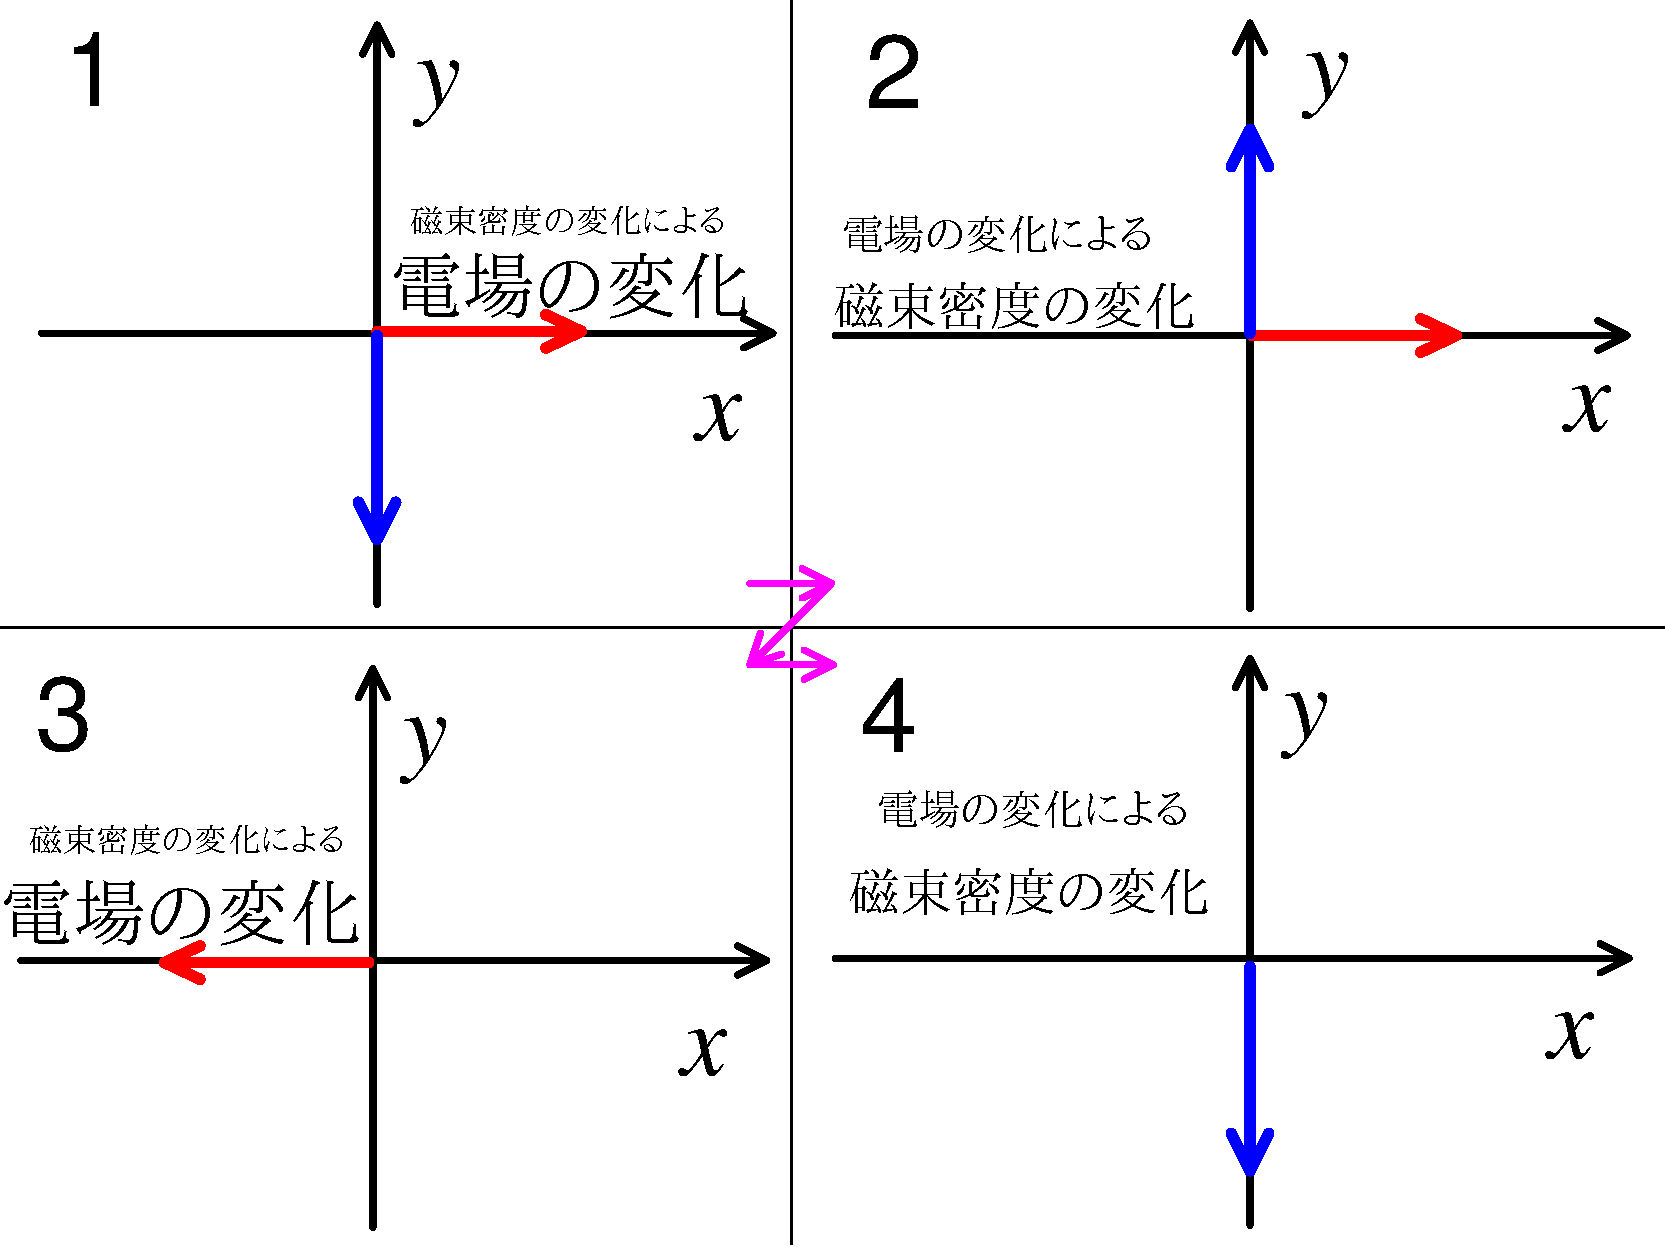
\includegraphics[keepaspectratio, width=6.5cm,height=6cm,clip]{denjiha1.pdf}
                        \caption{原点における電場と磁束密度の変化のイメージ}
                        \label{fig:denjiha1}
                \end{center}
            \end{figure}

            \begin{figure}[hbt]
                \begin{center}
                        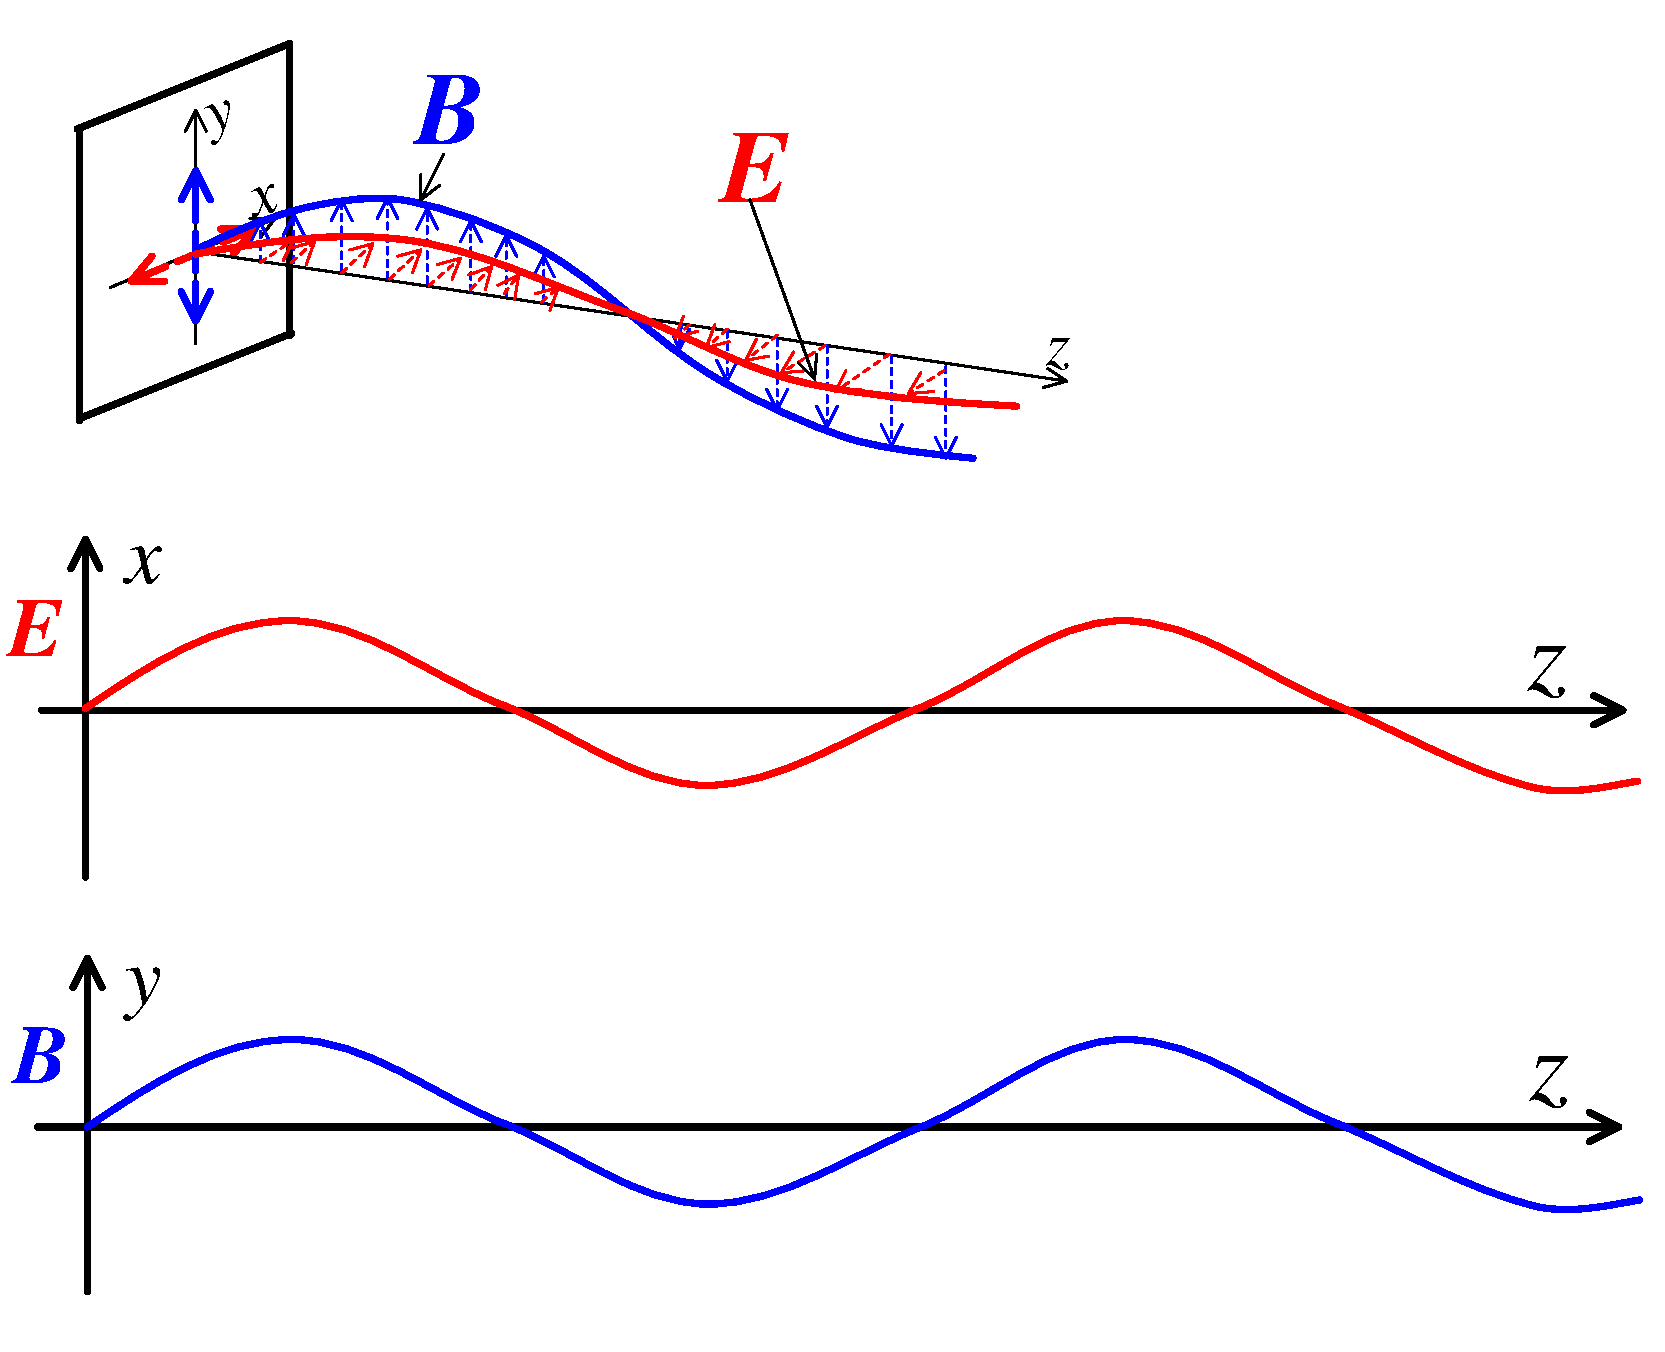
\includegraphics[keepaspectratio, width=6.5cm,height=6cm,clip]{denjiha2.pdf}
                        \caption{電磁波の伝搬のイメージ}
                        \label{fig:denjiha2}
                \end{center}
            \end{figure}

%   %==========================================================================
%   %  SubSection
%   %==========================================================================
    \subsection{電磁場のエネルギー と ポインティング・ベクトル}
        \begin{mycomment}
            電磁波は真空中を伝わる.となると,真空中にも電磁気的なエネルギーが
            蓄えられていると考えられよう.そこで,ここでは真空中に電磁波が存在しているとき,
            この空間に蓄えられている電磁気的なエネルギーについて考える.
        \end{mycomment}

        電磁場におけるエネルギー保存の法則を導く.

        ファラデーの電磁誘導の法則の両辺と,磁束密度 $\bB$ との内積をとり,
                                \begin{align}
                                \bB\cdot\left(\mathrm{rot\,} \bE \right)
                                &= \bB\cdot\left(-\frac{\rd \bB}{\rd t}\right).
                                \end{align}
        右辺を左辺に移項して整理すれば,
                                \begin{align}\label{eq:denyu11}
                                \bB\cdot\left(\frac{\rd \bB}{\rd t}
                                +\mathrm{rot\,} \bE\right)
                                &=0.
                                \end{align}

        次に,アンペール$=$マクスウェルの法則の両辺と,電場 $\bE$ の内積をとり,
                                \begin{align}\label{eq:MAs11}
                                \bE\cdot\mu_{0}\left(\bi+
                                \varepsilon_{0}\frac{\rd \bE}{\rd t}
                                \right)
                                &=\bE\cdot\left(\mathrm{rot\,}
                                \bB\right)
                                \notag \\
                                \Leftrightarrow \quad
                                \bE\cdot\left(
                                \varepsilon_{0}\mu_{0}\frac{\rd \bE}{\rd t}
                                -\mathrm{rot\,}\bB\right)
                                &=-\mu_{0}\bE\cdot\bi
                                \notag \\
                                \Leftrightarrow \quad
                                \bE\cdot\left(
                                \varepsilon_{0}\mu_{0}\frac{\rd \bE}{\rd t}
                                -\mathrm{rot\,}\bB\right)
                                &=-\mu_{0}\bE\cdot\bi
                                \end{align}
        とする.そして,式(\ref{eq:denyu11})と式(\ref{eq:MAs11})の両辺の和をとる.
                                \begin{align}
                                &-\mu_{0}\bE\cdot\bi \notag \\
                                &\quad =
                                \bB\cdot\left(\frac{\rd \bB}{\rd t}
                                +\drot \bE\right)
                                +\bE\cdot\left(
                                \varepsilon_{0}\mu_{0}\frac{\rd \bE}{\rd t}
                                -\drot \bB\right).
                                \end{align}
        右辺と左辺を入れ替えた
                \footnote{
                        A4紙の二段組にした場合,式が一行で納まらなかった.
                }.
            右辺を展開すると,
                                \begin{align}\label{elect_Energy1}
                                &-\mu_{0}\bE\cdot\bi \notag \\
                                &\quad =
                                \bB\cdot\frac{\rd \bB}{\rd t}
                                +\bB\cdot\drot\bE
                                +\bE\cdot\varepsilon_{0}\mu_{0}\frac{\rd \bE}{\rd t}
                                -\bE\cdot\drot\bB.
                                \end{align}

        ところで,任意のベクトル $\bX(t)$ に対して以下の式が成立する.
                                \begin{align}
                                \bX (t)\cdot\frac{\rd \bX (t)}{\rd t}=\frac{1}{2} \frac{\rd \bX(t)^{2}}{ \rd t} .
                                \end{align}
                                \begin{quotation}\small
                                                                なぜなら,
                                \begin{align*}
                                \frac{\rd \bX^{2}}{\rd t}&=\frac{\rd (\bX\cdot \bX)}{\rd t} \\ \notag \\ \notag
                                &=\bX\cdot\frac{\rd  \bX}{\rd t}+\frac{\rd  \bX}{\rd t}\cdot\bX \\ \notag \\ \notag
                                &=2\bX\cdot\frac{\rd \bX}{\rd t}\\ \notag \notag \\
                                \therefore\quad
                                \bX \cdot\frac{\rd \bX }{\rd t}&=\frac{1}{2} \frac{\rd \bX^{2}}{ \rd t} .
                                \end{align*}
                                \end{quotation}

        従って,式(\ref{elect_Energy1})の第1項と第3項を以下のように書き換えることができる.
                                \begin{align*}
                                &-\mu_{0}\bE\cdot\bi \notag \\
                                &\quad = \frac{1}{2} \frac{\rd \bB^{2}}{ \rd t}
                                +\bB\cdot\mathrm{rot\,} \bE
                                +\varepsilon_{0}\mu_{0}\frac{1}{2} \frac{\rd \bE^{2}}{ \rd t}
                                -\bE\cdot\mathrm{rot\,}\bB.
                                \end{align*}
        整理して,
                                \begin{align}
                                &-\mu_{0}\bE\cdot\bi \notag \\
                                &\quad = \frac{1}{2} \frac{\rd }{ \rd t}\left(\bB^{2}
                                +\varepsilon_{0}\mu_{0}\bE^{2}\right)
                                +\bB\cdot\mathrm{rot\,} \bE
                                -\bE\cdot\mathrm{rot\,}\bB.
                                \end{align}
        ここで,左辺の第3項と第4項は,以下のベクトル解析の恒等式を適用してまとめることができる.その公式とは,
        任意の2つのベクトル $\bX$,$\bY$ に対して,
                                \begin{align}
                                \bY\cdot\drot\bX - \bX\cdot\drot\bY =\ddiv(\bX\times\bY).
                                \end{align}
        この恒等式を,上式の左辺第3項と第4項に適用して,式変形すれば,
                                \begin{align}\label{eq:EB_energy}
                                \frac{1}{2} \frac{\rd}{\rd t}\left(\bB^{2}
                                +\varepsilon_{0}\mu_{0}\bE^{2}\right)
                                +\ddiv(\bE\times\bB)
                                =-\mu_{0}\bE\cdot\bi
                                \end{align}
        これを次のように書いてみる.
                                \begin{align}
                                        \ddiv(\bE\times\bB)
                                        + \frac{\rd}{\rd t}
                                          \left\{\frac{1}{2}
                                            \left(
                                              \bB^{2} + \varepsilon_{0}\mu_{0}\bE^{2}
                                            \right)
                                          \right\}
                                        = -\mu_{0}\bE\cdot\bi.
                                \end{align}
        さらに,
                \begin{align}
                        \bS &= \bE\times\bB \,,\,\\
                        W   &= \frac{1}{2} \left(\bB^{2}+\varepsilon_{0}\mu_{0}\bE^{2}\right)
                \end{align}
        と置くと,
            \begin{align}\label{eq:EB_energy}
                \ddiv \bS + \frac{\rd}{\rd t} W = -\mu_{0}\bE\cdot\bi.
            \end{align}
        こうしてみると,式の形が電荷保存の法則の式に似ている.電荷保存の法則は次のように記述された.
            \begin{align}
                 \ddiv\bi + \frac{\rd }{\rd t} \rho = 0.
            \end{align}
        電磁場のエネルギーの式(\ref{eq:EB_energy})の $\bS$ を
        電荷保存の法則の式の電流 $\bi$ と対応させて,
        また,$W$ の部分を電荷密度 $\rho$ と対応させて両式を比較してみよう.

        電荷保存の法則の式の意味は,「電荷の時間変化(つまり電荷の移動)が電流を発生させている」ということであった.
        これを電磁場のエネルギーの式に当てはめて考えると,
        $\left(\bB^{2}+\varepsilon_{0}\mu_{0}\bE^{2}\right)/2$ という
        量の時間変化が,$\ddiv(\bE\times\bB)$ という
        量を生じさせていることになる.また,右辺の電場と電流の積 $-\mu_{0}\bE\cdot\bi$ は
        電荷が電場より受ける単位時間あたりの仕事である.そこで,
        $\left(\bB^{2}+\varepsilon_{0}\mu_{0}\bE^{2}\right)/2$ を \textbf{電磁場のエネルギー密度},
        $\bE\times\bB$ を \textbf{ポインティング・ベクトル} とよぶことにすれば
            \footnote{
                ポインティング・ベクトル:\;Poynting vector であり,ポインティング(Poynting)は
                John Henry Poynting,(1852.9.9-- 1914.3.30,イギリス)
                という人の名前に由来する.
                pointingではない.
            },
        「電磁場のエネルギー密度の変化が,ポインティング・ベクトルを生じさせる」と
        表現される.




%===================================================================================================
%  Chapter : その他の電磁気学的現象
%  説明    : その他の電磁気現象を学習する.
%===================================================================================================
\chapter{その他の電磁気学的現象}
%   %-----------------------------------------------------------------------------------------------
%   %  Input
%   %    File Name : PhysNote_EM_2nd_Phenomenon.tex
%   %    説明      : その他の電磁気現象を学習する.
%   %                ・トムソン効果とか,ゼーベック効果とか,ゼーマン効果とか,いろいろ.
%   %-----------------------------------------------------------------------------------------------
        %===================================================================================================
%  Chapter : その他の電磁気学的現象
%  説明    : その他の電磁気現象を学習する.
%===================================================================================================
    %=======================================================================
    %  Section
    %=======================================================================
    \section{電気双極子}

    %=======================================================================
    %  SubSection
    %=======================================================================
    \section{熱電効果}
        %===================================================================
        %  SubSection
        %===================================================================
        \subsection{はじめに}
            ここでは,熱と電磁気とに関係する現象を考える.\textbf{熱電効果} と
            は,熱によって電流を生じさせる現象のことをいう.例えば,一様な物体
            があったとして,この物体の一部に熱を与えて,周囲よりも高温にしてみ
            る.この時,物体には温度勾配が生じる.熱い部分のエネルギーは冷たい
            う部分よりも高いので,当然,熱した部分の原子の持つ電子も,冷たい部
            分の電子よりも活発に運動していることだろう.活発な電子はその周囲に
            拡散することが容易に想像できる.この電子の拡散こそが,電流であり,
            熱電効果とよばれる理由である.

        %===================================================================
        %  SubSection
        %===================================================================
        \subsection{トムソン効果}\label{subsec:ThomsonEffect}

        %===================================================================
        %  SubSection
        %===================================================================
        \subsection{ペルチェ効果}

        %===================================================================
        %  SubSection
        %===================================================================
        \subsection{ゼーベック効果}

    %=======================================================================
    %  Section
    %=======================================================================
    \section{ゼーマン効果}\label{subsec:ZeemanEffect}
        原子にある程度エネルギーを与えると,その原子内の電子がエネルギー
        を吸収する.そして,電子のエネルギーがある一定値を超えると,エネル
        ギーを抱えきれなくなり,電磁波としてそれを放出する.このとき放出さ
        れる電磁波の波長は原子ごとに決まっている.一般に,放出される電磁波
        の波長は複数である.つまり,原子はエネルギーを外部から与えると,決
        まったいくつかの波長の電磁波を放出する.この原子が出す複数の波長の
        電磁波のことを,\textbf{原子スペクトル} という.また,そのひとつひ
        とつを \textbf{原子スペクトル線} という.

        単一の波長しか放出しない原子
            \footnote{
                スペクトル線をひとつしか持たない原子のこと.
            }
        も存在する.しかし,磁束密度中でエネルギー
        を与えた場合,それが複数種類の電磁波を放出するようになる
            \footnote{
                スペクトル線が2つ以上に分裂するということ.
            }.
        この現象を \textbf{ゼーマン効果} という.

    %=======================================================================
    %  Section
    %=======================================================================
    \section{電子の実験的発見}
        電子は,どのようにしてその存在が認められたのだろうか.
            \begin{figure}[hbt]
                \begin{center}
                    \includegraphicslarge{ThomomExpElec001.pdf}
                    \caption{トムソンの陰極線の実験}
                    \label{fig:ThomomExpElec001}
                \end{center}
            \end{figure}




%===================================================================================================
%  Chapter : 共変形式のマクスウェル方程式
%  説明    : マクスウェル方程式を,ベクトルポテンシャルA とスカラーポテンシャルphi を
%            用いて表す.また,ゲージ変換についても考える.特殊相対性理論への導入も,
%            マクスウェル方程式のガリレイ変換ができないことを通して,行う.
%            その後,電磁ポテンシャルを導入し,マクスウェル方程式を共変形式に書き換える.
%===================================================================================================
\chapter{共変形式のマクスウェル方程式}
%   %-----------------------------------------------------------------------------------------------
%   %  Input
%   %    File Name : PhysNote_EM_2nd_Potential.tex
%   %    説明      : 量子力学や相対性理論に馴染みやすいように,
%   %                マクスウェル方程式をポテンシャル表示に書き換える.
%   %-----------------------------------------------------------------------------------------------
        %===================================================================================================
%  Chapter : マクスウェル方程式のポテンシャル表示
%  説明    : マクスウェル方程式を,ベクトルポテンシャルA とスカラーポテンシャルphi を
%            用いて表す.また,ゲージ変換についても考える.特殊相対性理論への導入も,
%            マクスウェル方程式のガリレイ変換ができないことを通して,行う.
%===================================================================================================
%   %==========================================================================
%   %  Section
%   %==========================================================================
    \section{ポテンシャルの導入}
        \begin{mycomment}
            電磁気学を相対性理論や量子力学で扱うとき,
            電場や磁束密度をそのままの形で表現するよりも,
            ポテンシャルを用いて表現したほうが
            都合がよい.そこでここでは,
            電場と磁束密度をポテンシャル表記することを考える.

            その方法は,まず,磁束密度に対するガウスの法則から,
            ベクトルポテンシャルを定義 $\bA$ し,
            この $\bA$ によって,磁束密度を
            表現することを考える.
            そして,ベクトルポテンシャルによって表現された
            磁束密度を電磁誘導の法則に代入することにより,
            電場のポテンシャル表記する.このとき,電位(電気的なスカラーポテンシャル)と電場の関係
            を考慮する必要がある.
        \end{mycomment}
%       %======================================================================
%       %  SubSection
%       %======================================================================
        \subsection{スカラーポテンシャル:$\phi$}
            スカラーポテンシャルとは,電位 $\phi$ のことである.
            これから,マクスウェル方程式を $\phi$ を用いた表現に書き直すことを
            試みる.

%       %======================================================================
%       %  SubSection
%       %======================================================================
        \subsection{ベクトルポテンシャル:$\bA$}
            ポテンシャルを用いて電場や磁束密度を表現することを考える.
            まず,磁束密度について考える.磁束密度は,
            ガウスの法則により,$\mathrm{div\,}\bB=0$ を満たしている.
            このことに注目しながら,次のベクトル解析の恒等式を考える.
            あるベクトル $\bA$ に対して,
            \begin{align}\label{div_rot}
            \mathrm{div\,rot\,}\bA=0
            \end{align}
            回転の発散は常に 0 であるということを意味している.式(\ref{div_rot})の
            ベクトル $\mathrm{rot\,}\bA$ を
            磁束密度 $\bB$ に置き換えれば,
            すなわち,
            \begin{align}\label{rotA}
            \bB=\mathrm{rot\,}\bA
            \end{align}
            とすれば,
            以下の恒等式を
            得られる.
            \begin{align}\label{div_rotA}
            \mathrm{div\,}\bB=0
            \end{align}
            式(\ref{rotA})のように磁束密度を表すことによって,
            ガウスの法則が数学的に自動的に成り立つのである.
            この式(\ref{rotA})を満たすようなベクトル $\bA$ の
            ことを \textbf{ベクトルポテンシャル} という.

            物理的には,ベクトルポテンシャルという概念を
            理解することは難しいが,ポテンシャルを
            基礎に置いた理論は現代では主流である.
            解析力学,量子力学や相対性理論との関連を考えるとき,
            ベクトルポテンシャルの概念は便利な道具として用いられる.
            ベクトルポテンシャルの実在性は,\textbf{Aharonov=Bohm効果} という
            現象によって確認されている.この効果については,量子力学の
            知識が必要である.

%       %======================================================================
%       %  SubSection
%       %======================================================================
        \subsection{ベクトルポテンシャル $\bA$ の形}
            前項目では,ベクトルポテンシャル $\bA$ を磁束密度がガウスの法則を満たすように定義したが,
            具体的な形はまだわかっていない.$\bA$ は電流 $\bi$ と 位置 $\br$ で表せる.
            以下で計算し,確認してみよう.

            ベクトルポテンシャル $\bA$ の定義は磁束密度 $\bB$ に対するガウスの法則から
            定義された.
                \begin{equation*}
                    \bB := \drot \bA
                \end{equation*}
            ところで,磁束密度はビオ$=$サバールの法則によって記述される.
            そこで,ビオ$=$サバールの法則を式変形していき,
            上の磁束密度とベクトルポテンシャルの関係式の形へ誘導し,
            ベクトルポテンシャルに対応する部分を見ることで,ベクトルポテンシャルの形を考えていく.

            最初に,式変形につかう公式を2つ確認する.
            一つは $\br'$ に関する $\dgrad$ として,
                \begin{align}\label{eq:grad_r}
                    \dgrad_{\br'} \left( \frac{1}{| \br -\br' |}\right)
                    =-\frac{\br-\br'}{| \br-\br' |^{3}}.
                \end{align}
            もう一つは,sを任意のスカラー
                \footnote{
                    スカラーとは,大きさのみを数である.
                    ベクトルが複数の数の組みで表現されるのに対し,
                    スカラーは1つの数で表現される.
                }
            ,$\bU$ を任意のベクトルとして,
                \begin{align}\label{eq:grad_sU0}
                    \drot(s\bU\,) = s\,\drot\bU - \bU\times(\dgrad s)
                \end{align}
            というベクトル解析の公式である.今回はこの公式の $\bU$ は
            定電流 $\bi(\br)$ に対応させるので,定数ベクトルとして
            の扱いになる.$\bU$ を定数ベクトルと見たとき,この公式(\ref{eq:grad_sU0})は
            次のように計算される.
                \begin{align}\label{eq:grad_sU}
                    \drot(s\bU\,) = - \bU\times(\dgrad s).
                \end{align}
            今回の式変形では公式を変形した式(\ref{eq:grad_sU})を
            用いる.

            それでは,式変形に執りかかろう.
            ビオ$=$サバールの法則は以下のようであった.
                \begin{align*}
                    \bB(\br)
                    &=\frac{\mu_{0}}{4\pi}
                    \int\frac{\bi(\br')\times
                    (\br-\br')
                    }{|\br-\br'|^{3}}\df V' \\
                    &=\frac{\mu_{0}}{4\pi}
                    \int\bi(\br')\times
                    \frac{\br-\br'}
                    {|\br-\br'|^{3}}\df V'
                \end{align*}
            一番右の式に先ほどの公式(\ref{eq:grad_r})を用いると,
                \begin{align}
                    \bB(\br)
                    =-\frac{\mu_{0}}{4\pi}
                    \int\bi(\br')\times
                    \dgrad_{\br'} \left( \frac{1}{| \br -\br'|}\right)
                    \df V'
                \end{align}
            右辺に,先ほど記述したベクトル解析の公式 $\drot(s\bU\,) = - \bU\times(\dgrad s)$ を
            使うと,
                \begin{align}\label{eq:vector_Pt_A}
                    \bB(\br)
                    &=\int \drot \frac{\mu_{0}}{4\pi}\frac{\bi(\br\,')}{| \br -\br'|}\df V' \notag \\
                    &=\drot \int \frac{\mu_{0}}{4\pi}\frac{\bi(\br\,')}{| \br -\br'|}\df V'
                \end{align}
            となる.この式(\ref{eq:vector_Pt_A})と,ベクトルポテンシャルと磁束密度の関係式 $\bB=\drot\bA$ の
            ベクトルポテンシャル $\bA$ に対応する部分に注目すれば,
                \begin{align}
                    \bA(\br)
                    =\int\frac{\mu_{0}}{4\pi}\frac{\bi(\br\,')}{| \br -\br'|}\df V'
                \end{align}
            を得る.以上で,ベクトルポテンシャルの具体的な形を得ることができた.

%       %======================================================================
%       %  SubSection
%       %======================================================================
        \subsection{磁束密度のポテンシャル表示}
            今までの議論で,散々書かれてきたが,改めて記載しておこう.
            磁束密度 $\bB$ は,ベクトルポテンシャル $\bA$ を用いると,以下のように
            表現できる.
                \begin{align}
                    \bB = \drot \bA.
                \end{align}

%       %======================================================================
%       %  SubSection
%       %======================================================================
        \subsection{電場のポテンシャル表示}
            前項目では,磁束密度をベクトルポテンシャルを用いて
            表現することを考えた.それは,$\bB=\mathrm{rot\,}\bA$ の
            様に表現される.さて,ここでは電場をポテンシャルで表現することを考える.
            そのためは,$\bB=\mathrm{rot\,}\bA$ を用いる.
            どう用いるかといえば,この式をファラデーの電磁誘導の法則に代入するのである.
            ファラデーの電磁誘導の法則は
            \begin{align}
            \drot \bE &= -\frac{\rd \bB}{\rd t}
            \end{align}
            であった.この式に $\bB=\mathrm{rot\,}\bA$ を
            代入すると,
            \begin{align}
            \mathrm{rot\,} \bE &= -\frac{\rd(\mathrm{rot\,}\bA)}{\rd t}\notag \\ \notag \\
            \Leftrightarrow
            \mathrm{rot\,}\frac{\rd\bA}{\rd t}
            +\mathrm{rot\,} \bE&=0 \notag \\
            \Leftrightarrow
            \mathrm{rot\,}\left(\frac{\rd\bA}{\rd t}
            + \bE\right) &=0
            \end{align}
            となる.一般的に,この式の解は
            \begin{align}
            \frac{\rd\bA}{\rd t}
            + \bE&=-\mathrm{grad\,}\phi
            \end{align}
            と書かれる.但し数学的には,右辺の負符号は必要ない.負の符号を付けたのは,
            電位の定義によるものである.
            従って,電場をポテンシャル表示すると,
            \begin{align}
            \bE&=-\frac{\rd\bA}{\rd t}-\mathrm{grad\,}\phi
            \end{align}
            となる.


%   %==========================================================================
%   %  Section
%   %==========================================================================
    \section{マクスウェル方程式のポテンシャル表示}
    \begin{mycomment}
            さて,以上の計算から,電場と磁束密度の
            ポテンシャル表示を確認した.具体的には,
            電場と磁束密度はそれぞれ,
            スカラーポテンシャル $\phi$ とベクトルポテンシャル $\bA$ を
            用いて,
            \begin{align}\label{pt_EB}
            \begin{cases}
            \displaystyle\bE=-\frac{\rd\bA}{\rd t}-\dgrad\phi \\  \notag \\
            \vspace{2mm}
            \displaystyle\bB=\drot\bA
            \end{cases}
            \end{align}
            のように表現されることが分かった.
            このポテンシャル表示が示すように,電場や磁束密度はポテンシャルから導かれると
            考えることも可能である.

            このポテンシャル表示を導く課程で,ファラデーの電磁誘導の法則と
            磁束密度に対するガウスの法則を用いた.そして,マクスウェル方程式の残りの
            もう二つの法則,すなわち,アンペール$=$マクスウェルの法則と電場に対するガウスの法則
            のそれぞれに,上で確認した電場と磁束密度を代入すれば,
            それによって得た方程式と式(\ref{pt_EB})はマクスウェル方程式と
            同等であると考えられる.では,実際に計算していくことにする.
    \end{mycomment}


%       %======================================================================
%       %  SubSection
%       %======================================================================
        \subsection{アンペール$=$マクスウェルの法則の変形}
            アンペール$=$マクスウェルの法則は以下のように書かれることは前に確認した.
            すなわち,
            \begin{align}
            \left(\bi+
            \varepsilon_{0}\frac{\rd \bE}{\rd t}
            \right)
            =\frac{1}{\mu_{0}}\drot\bB
            \end{align}
            である.この方程式に,電場や磁束密度のポテンシャル表示式(\ref{pt_EB})を
            考慮すると,以下のようになる.
            \begin{align}\label{AM_phi_A}
            \bi+
            \varepsilon_{0}\frac{\rd }{\rd t}
            \left( -\frac{\rd\bA}{\rd t}-\dgrad\phi\right)
            =\frac{1}{\mu_{0}}\drot\left(\drot\bA\right)
            \end{align}

            さてここで,ベクトル解析による恒等式を用いる.それは,任意のベクトルを $\bC$ としたとき,
            \begin{align}\label{rotrot_C_gdCdgC}
            \drot\drot\bC:=
           \dgrad\ddiv\bC - \Delta \bC
            \end{align}
            が成り立つというものである.この恒等式(\ref{rotrot_C_gdCdgC})を
            用いれば,式(\ref{AM_phi_A})は
            \begin{align}
            &\frac{1}{\mu_{0}}\left(\dgrad\ddiv\bA - \Delta \bA\right) \notag \\
            &\quad=\bi+ \varepsilon_{0}\frac{\rd }{\rd t} \left( -\frac{\rd\bA}{\rd t}-\dgrad\phi\right) \notag \\
            &\Leftrightarrow -\mu_{0}\bi \notag \\
            &\quad=\left(\Delta -\frac{1}{c^{2}}\frac{\rd^{2}}{\rd t^{2}}\right)\bA
             -\mathrm{grad\,}\left( \ddiv\bA + \frac{1}{c^{2}}\frac{\rd \phi}{\rd t}\right)
            \end{align}
            と変形される.ここで,$c=1/\sqrt{\varepsilon_{0}\mu_{0}}$ とおいた.
            $c$ は波動の位相速度で,特にこの場合は光速の意味を持つ.
            注意しておくことは,
            この式はもはやアンペール$=$マクスウェルの法則を
            示すものではないということである.

%       %======================================================================
%       %  SubSection
%       %======================================================================
        \subsection{電場に対するガウスの法則の変形}
            電場に対するガウスの法則を書き下すと,
            \begin{align}
            \ddiv\bE
            =\frac{1}{\varepsilon_{0}}\rho
            \end{align}
            である.この式に,ポテンシャル表示された
            電場 $\displaystyle\bE = -(\rd\bA/\rd t) -\mathrm{grad\,}\phi$ を
            代入すると,
            \begin{align}
            \ddiv\left(-\frac{\rd\bA}{\rd t}-\mathrm{grad\,}\phi\right)
            =\frac{1}{\varepsilon_{0}}\rho \notag \\  \notag \\
            \Leftrightarrow
            -\frac{\rd(\mathrm{div\,}\bA)}{\rd t}-\mathrm{div\,grad\,}\phi
            =\frac{1}{\varepsilon_{0}}\rho
            \end{align}
            そして,$\Delta:=\mathrm{div\,grad\,}$ ということに注意すれば,
            \begin{align}
            \frac{\rd(\mathrm{div\,}\bA)}{\rd t}+\Delta\phi
            =-\frac{1}{\varepsilon_{0}}\rho
            \end{align}
            となる.ここで,少々トリッキーな操作を行う.
            この式の両辺に $-\varepsilon_{0}\mu_{0}(\rd^{2} \phi/\rd t^{2})$ を加える.
            \begin{align}
            &\frac{\rd(\mathrm{div\,}\bA)}{\rd t}+\Delta\phi
            -\varepsilon_{0}\mu_{0}\frac{\rd^{2} \phi}{\rd t^{2}}
            =-\frac{1}{\varepsilon_{0}}\rho -\varepsilon_{0}\mu_{0}\frac{\rd^{2} \phi}{\rd t^{2}}\notag \\ \notag \\
            &\Leftrightarrow\,
            \left(\Delta
            -\frac{1}{c^{2}}\frac{\rd^{2} }{\rd t^{2}}\right)\phi
            +\frac{\rd}{\rd t}\left(\mathrm{div\,}\bA
            +\frac{1}{c^{2}}\frac{\rd \phi}{\rd t}
            \right)
            =-\frac{1}{\varepsilon_{0}}\rho
            \end{align}

            これで,とりあえずの式変形が終了した.この後に,
            これら4つの式を,次に確認する \textbf{Lorentz ゲージ} という
            ゲージを導入し,もう少し表現を簡略化する.その前に,とりあえず
            今までに得られたマクスウェル方程式と等価な方程式をまとめておく.
                    \begin{myshadebox}{マクスウェル方程式のポテンシャル表示}
                        以下の方程式群は,マクスウェル方程式を,ベクトルポテンシャルと
                        スカラーポテンシャルを用いた表現に書きなおしたものであり,
                        先に導出したマクスウェル方程式と(数学的に)同等の内容である.
                        \begin{align}
                            \bE&=-\displaystyle
                            \frac{\rd\bA}{\rd t}-\mathrm{grad\,}\phi \\ \notag \\
                            \vspace{2mm}
                            \bB&=\mathrm{rot\,}\bA
                        \end{align}
                        \begin{align}
                            &-\mu_{0}\bi  \\\,\vspace{2mm}  \notag \\
                            &=\left(\Delta
                            -\frac{1}{c^{2}}\frac{\rd^{2}}{\rd t^{2}}\right)\bA
                            -\mathrm{grad\,}\left( \mathrm{div\,}\bA
                            +\frac{1}{c^{2}}\frac{\rd{\phi}}{\rd t}\right) \\
                            &-\frac{1}{\varepsilon_{0}}\rho \notag \\
                            &=\left(\Delta
                            -\frac{1}{c^{2}}\frac{\rd^{2} }{\rd t^{2}}\right)\phi
                            +\frac{\rd}{\rd t}\left(\mathrm{div\,}\bA
                            +\frac{1}{c^{2}}\frac{\rd \phi}{\rd t}
                            \right)
                        \end{align}
                    \end{myshadebox}

                このままでは式の形がややこしいので,
                次に \textbf{ゲージ変換} を確認して,
                \textbf{ローレンツ条件} を導入しよう.


%       %======================================================================
%       %  SubSection
%       %======================================================================
        \subsection{ゲージ変換}
            電場 $\bE$ と磁束密度 $\bB$ のポテンシャル表示の式は以下のように表現されることは,
            前項目で既に確認している.
                    \begin{align}
                            \bE&=-\displaystyle
                            \frac{\rd\bA}{\rd t}-\mathrm{grad\,}\phi \\  \notag \\
                            \vspace{2mm}
                            \bB&=\mathrm{rot\,}\bA
                    \end{align}
            ここで,2つのポテンシャル $\bA$ と $\phi$ を以下のように変換してみる.\\
                        \begin{myshadebox}{ゲージ変換}
                            2つのポテンシャル $\bA$ と $\phi$ の \textbf{ゲージ変換} とは,
                            以下の変換のことをいう.
                            \begin{align}\label{guage1}
                                \bA'&=\bA-\dgrad\chi \\ \notag \\
                                \phi ' &=\phi +\frac{\rd \chi}{\rd t}
                            \end{align}
                        \end{myshadebox}

            ここで,$\chi$ は任意の関数である.
            このように,ポテンシャルを式(\ref{guage1})で変換することを,\textbf{ゲージ変換} という.
            なぜこんな可笑しな変換を考えるかといえば,それは次のような理由による.
            \textbf{ポテンシャルをゲージ変換しても,
            電場と磁束密度は形を変えない}.このことを確認をしておこう.

            まず,電場について考えよう.ゲージ変換をしたポテンシャルでの電場 $\bE\,'$ は,
                    \begin{align}
                            &\bE\,' \notag \\
                            &=-\displaystyle \frac{\rd\bA'}{\rd t}-\mathrm{grad\,}\phi ' \notag \\
                            &=-\frac{\rd}{\rd t}\left( \bA-\dgrad\chi \right)
                            -\dgrad\left( \phi+\frac{\rd \chi}{\rd t} \right) \notag \\
                            &=-\frac{\rd  \bA}{\rd t}+\frac{\rd  (\dgrad\chi)}{\rd t}
                            -\dgrad\phi-\dgrad\left( \frac{\rd \chi}{\rd t} \right) \notag \\
                            &=-\frac{\rd  \bA}{\rd t}+-\dgrad\left( \frac{\rd \chi}{\rd t} \right)
                            -\dgrad\phi-\dgrad\left( \frac{\rd \chi}{\rd t} \right) \notag \\
                            &=-\frac{\rd  \bA}{\rd t}-\dgrad\phi \notag \\
                            &=\bE\notag \\ \notag \\
                            &\therefore\,\,\bE\,'=\bE
                    \end{align}
            よって,ゲージ変換を適用しても,電場の形の変化はない.

            次に,磁束密度について確認しよう.ゲージ変換された磁束密度を $\bB\,'$ とすると,
                    \begin{align}
                    \bB\,'&=\drot\bA' \notag \\
                    &=\drot\left(\bA-\mathrm{grad \chi} \right)\notag \\
                    &=\drot\bA-\mathrm{rot\,grad} \,\chi\notag \\
                    &=\drot\bA\notag \\
                    &=\bB\notag \\
                    \therefore\,\quad\,
                    \bB\,'&=\bB
                    \end{align}
            よって電場と同様に,磁束密度についてもゲージ変換を適用しても,磁束密度の形を変えることはないことが示された.

            以上のように,電場と磁束密度はゲージ変換に対してその形を変化させることは
            ないことを示したが,このことを,電場と磁束密度は \textbf{ゲージ変換に対して不変である} と表現する.

%       %======================================================================
%       %  SubSection
%       %======================================================================
        \subsection{ローレンツ条件}
            ベクトルポテンシャルとスカラーポテンシャルが以下の式ローレンツ条件を満たすと仮定する.
                        \begin{myshadebox}{ローレンツ条件式}
                            \begin{align}
                                \mathrm{div\,}\bA + \frac{1}{c^{2}}\frac{\rd \phi}{\rd t}
                                =0
                            \end{align}
                        \end{myshadebox}

            こうすると,マクスウェル方程式がきれいに整理される.しかし,
            上のローレンツ条件はどうなるか.実は,これは大した問題ではなく,理論にも矛盾を
            引き起こしたりしない.そのことを確認するため,計算してみよう.

            ローレンツ変換式に,ゲージ変換した
            ポテンシャル $\bA'=\bA-\dgrad\chi$,
            $\phi ' =\phi +\left(\rd \chi/\rd t\right)$ を代入して,
                            \begin{align*}
                                &\mathrm{div\,}\bA' + \frac{1}{c^{2}}\frac{\rd \phi '}{\rd t} \notag \\
                                &\quad=\mathrm{div\,}(\bA-\dgrad\chi)
                                +\frac{1}{c^{2}}\frac{\rd}{\rd t}
                                \left(\phi +\frac{\rd \chi}{\rd t}\right) \\ \notag \\
                                &\quad=\mathrm{div\,}\bA
                                -\mathrm{div\,grad\,}\chi
                                +\frac{1}{c^{2}}\frac{\rd \phi}{\rd t}
                                +\frac{1}{c^{2}}\frac{\rd^{2} \chi}{\rd t^{2}} \\ \notag \\
                                &\quad=\mathrm{div\,}\bA
                                +\frac{1}{c^{2}}\frac{\rd \phi}{\rd t}
                                \left(
                                    -\mathrm{div\,grad\,}\chi
                                +\frac{1}{c^{2}}\frac{\rd^{2} \chi}{\rd t^{2}}
                                \right)
                            \end{align*}
            ここで,$\Delta:=\mathrm{div\,grad\,}$ であることに注意して,
                            \begin{align*}
                                &\mathrm{div\,}\bA'
                                +\frac{1}{c^{2}}\frac{\rd \phi '}{\rd t} \\
                                &\quad=
                                \mathrm{div\,}\bA
                                +\frac{1}{c^{2}}\frac{\rd \phi}{\rd t}
                                -\left(
                                    \Delta\chi
                                -\frac{1}{c^{2}}\frac{\rd^{2} \chi}{\rd t^{2}}
                                \right)
                            \end{align*}
            この式で右辺第1項と第2項の和は,ローレンツ条件で 0になるから,
                            \begin{align*}
                                \mathrm{div\,}\bA'
                                +\frac{1}{c^{2}}\frac{\rd \phi '}{\rd t}
                                &=
                                -\left(
                                    \Delta\chi
                                -\frac{1}{c^{2}}\frac{\rd^{2} \chi}{\rd t^{2}}
                                \right)
                            \end{align*}
            と計算される.ゲージ変換しても,ローレンツ変換式を維もできるためには,この式の右辺が0に等しければよく,
            つまり
                            \begin{align}
                                \left(
                                    \Delta\chi
                                -\frac{1}{c^{2}}\frac{\rd^{2} \chi}{\rd t^{2}}
                                \right)
                                =0
                            \end{align}
            が満たされていればよい.この条件を満たすような解 $\chi$ は1つ以上,すなわち,
            複数存在する.しかし,この条件を満たすような解ならば,
            $\chi$ はどのようなものであってもよい.とにかく,そのような解が存在するということを
            確認できればそれでよいのである.
            解である $\chi$ 具体的な形はあまり本質的ではないのだ.以上で確認終了.
            これで安心してローレンツ条件を用いることができる.


            この条件式を用いて,ポテンシャル表記されたマクスウェル方程式
            を整理するとつぎのようになる.
               \begin{myshadebox}{マクスウェル方程式のポテンシャル表示}
                        \begin{align}
                            \bE&=-\displaystyle
                            \frac{\rd\bA}{\rd t}-\mathrm{grad\,}\phi \\ \notag \\
                            \vspace{2mm}
                            \bB&=\mathrm{rot\,}\bA
                    \end{align}
                    \begin{align}
                            \left(\Delta
                            -\frac{1}{c^{2}}\frac{\rd^{2}}{\rd t^{2}}\right)\bA
                            &=-\mu_{0}\bi  \\\,\vspace{2mm} \notag \\
                            \left(\Delta
                            -\frac{1}{c^{2}}\frac{\rd^{2} }{\rd t^{2}}\right)\phi
                            &=-\frac{1}{\varepsilon_{0}}\rho
                    \end{align}
                        \textbf{ローレンツ条件式}
                            \begin{align}
                                \mathrm{div\,}\bA
                                +\frac{1}{c^{2}}\frac{\rd \phi}{\rd t}
                                =0
                            \end{align}
               \end{myshadebox}


                    条件式が1つ多くなるが,マクスウェル方程式はかなり整理された形になったと
                    感じられることと思う(感覚は人それぞれではあるが...)
                      \footnote{
                        くどいようだが,確認しておきたいことがある.式を1つ追加してまでも
                        マクスウェル方程式をポテンシャル表記するのは,後に考える量子力学や相対性理論との
                        かかわりをより深く理解するためである.この理由を改めておくのは,学習意欲を
                        失うことのないようにするためである.
                      }.


%       %======================================================================
%       %  SubSection
%       %======================================================================
        \subsection{ポテンシャル表記の利点}
                    マクスウェル方程式を,電位 $\phi$ とベクトルポテンシャル $\bA$ で
                    表すことで,マクスウェル方程式が数学的に美しい形で表現された.
                    つまり,方程式が解きやすくなったのだ.マクスウェル方程式を解くとは,
                    電場 $\bE$ と磁束密度 $\bB$ を求めることである.元の式で
                    は,$\bE$ と $\bB$ がひとつの方程式に混在している.
                    それに対して,ポテンシャル表記された方程式は,$\phi$ と $\bA$ が
                    分離されている.つまり,元の式から $\bE$,$\bB$ を解くより,
                    ポテンシャル表記された方程式から $\phi$,$\bA$ を求める
                    方が簡単なのである.$\phi$ と $\bA$ さえ求まれば,$\bE$ と $\bB$ は
                    すぐに求められる.数学的解析を行いたい場合には,この
                    ポテンシャル表記された方程式は,とても役に立つ.

                    さらに言えば,ポテンシャル表記された方程式は
                    量子力学や相対性理論との相性がいい.量子力学・
                    相対性理論を学ぶ際には,ポテンシャル表記の方程式を
                    理解していなければならない.

                    もちろん,数式と物理現象との対応を,鮮やかに表現しているのは
                    元の $\bE$ と $\bB$ で表される方程式である.
                    要するに,目的応じて数式的表現を選べるのである.
                    実際の物理現象のイメージを大切にしたい場合は $\bE$ と $\bB$ で
                    表される方程式を使えばいい.
                    問題を解析的(数学的)に解きたい場合はポテンシャル表記の方程式を
                    選べばよい.一度数式で表現された物理現象は,もはや物理現象の
                    数式表現と言うことにとどまらず,純粋に数学的な方程式の問題としても
                    見れるのである.ポテンシャル表記された方程式は,意味がわからないとして
                    避けてしまってはならない.むしろ,これから先の学習で,ポテンシャル
                    表記の方程式はなくてはならないものになるはずである.



%   %-----------------------------------------------------------------------------------------------
%   %  Input
%   %    File Name : PhysNote_EM_2nd_ToSpecialRelativity.tex
%   %    説明      : マクスウェル方程式の共変形式表示への導入
%   %-----------------------------------------------------------------------------------------------
        %===================================================================================================
%  Chapter : マクスウェル方程式のポテンシャル表示
%  説明    : マクスウェル方程式を,ベクトルポテンシャルA とスカラーポテンシャルphi を
%            用いて表す.また,ゲージ変換についても考える.特殊相対性理論への導入も,
%            マクスウェル方程式のガリレイ変換ができないことを通して,行う.
%===================================================================================================
%   %==========================================================================
%   %  Section
%   %==========================================================================
    \section{マクスウェル方程式のガリレイ変換}
        \subsection{マクスウェル方程式に対してガリレイ変換は適用できない}
            マクスウェル方程式をガリレイ変換すると,式の形が変わってしまう.
            つまり,残念ながら,マクスウェル方程式はガリレイ変換に対して不変でない.

            式で示すと,S座標系と S'座標系で式の形が違うということであり,
                \[
                {\nabla}^{2} -\frac{1}{{c}^{2}}\frac{{\rd}^{2}}{{\rd t}^{2}}
                \neq
                {\nabla '}^{2} -\frac{1}{{c}^{2}}\frac{{\rd}^{2}}{{\rd t'}^{2}}
                \]
            ということ.要するに,波動方程式はガリレイ変換にできないので,
            波動方程式をその内部に含むマクスウェル方程式もガリレイ変換に従わないということだ.

            しかし,マクスウェル方程式が間違っているのではない.
            マクスウェル方程式は電磁波など現象を予言できるし,
            電磁気現象を十分に説明できる方程式であり,誤っているとは考えにくい.

            では,何がおかしいのか.実は,そもそも,ガリレイ変換がおかしいのである.
            特殊相対性理論により,ガリレイ変換は,光速よりも十分に遅く等速運動する物体に
            対して有効な変換であることが分かった.より一般的な変換法則はローレンツ変換
            であり,ガリレイ変換はローレンツ変換の特殊な場合
                \footnote{
                    ここでいう特殊な場合とは,光速に対して,とても遅く運動するという状況である.
                }
            に過ぎない.そして,マクスウェル方程式はローレンツ変換に対しては不変である.

            以下で,このことを数式を使いながら考えていこうと思う.
            よく教科書では,
                1) ガリレイ変換を偏微分の公式に形を変えて,
            その後に,
                 2) 電磁波の波動方程式がその偏微分で表されたガリレイ変換の式に不変でないことを示している.
            このノートでも同じような手法をとる.計算課程も詳しく記載しておこう
                \footnote{
                    多くの教科書では,計算が当たり前すぎるためなのか,紙面の都合上の問題なのか,
                    計算過程が示されておらず,結果のみが記されている.
                }.

        \subsection{ガリレイ変換と偏微分演算子}
            \subsubsection{時間微分の計算}
                座標変換により,$S=S'(x',\,t')$ と変換できるとする.
                このとき,合成関数の微分を用いると,\textbf{時間微分} は以下の通り.
                    \begin{align*}
                        \frac{\rd S }{\rd t'} &=   \frac{\rd S }{\rd x } \frac{\rd x }{\rd t'}
                                                + \frac{\rd S }{\rd t } \frac{\rd t }{\rd t'} \\
                                            &=   \frac{\rd x }{\rd t'} \frac{\rd S }{\rd x }
                                                + \frac{\rd t }{\rd t'} \frac{\rd S }{\rd t } \\
                                            &=   \left(
                                                \frac{\rd x }{\rd t'} \frac{\rd   }{\rd x }
                                                + \frac{\rd t }{\rd t'} \frac{\rd   }{\rd t }
                                                \right) S.
                    \end{align*}

                ガリレイ変換の場合,空間座標は $x=x'+Vt'$($V$ は S系と S'系の相対速度)なので,
                    \begin{align*}
                        \frac{\rd x }{\rd t'} = \frac{\rd }{\rd t'} \left( x'+Vt' \right)
                                              = V.
                    \end{align*}
                さらに,
                    \begin{align*}
                        \frac{\rd x}{\rd x'}  = \frac{\rd }{\rd x'} \left( x'+Vt' \right)
                                              = 1
                    \end{align*}
                が成立する.従って,
                    \begin{align*}
                        \frac{\rd S }{\rd t'} &=   \left(
                                                  \frac{\rd x }{\rd t'} \frac{\rd   }{\rd x }
                                                + \frac{\rd t }{\rd t'} \frac{\rd   }{\rd t }
                                                  \right) S \\
                                              &=   \left(
                                                  V \frac{\rd   }{\rd x }
                                                + 1 \frac{\rd   }{\rd t }
                                                  \right) S.
                    \end{align*}
                微分演算子の部分を抽出すると(両辺の $S$ の記述を省略すると)
                    \begin{align}
                        \frac{\rd  }{\rd t'} =  V \frac{\rd   }{\rd x } + \frac{\rd   }{\rd t }
                    \end{align}
                を得る.よく見る式が現れた.

                $y$ と $z$ も同様に(書くまでもない気がするが),
                    \begin{align}
                        \frac{\rd  }{\rd t'} &=  V \frac{\rd   }{\rd y } + \frac{\rd   }{\rd t } \\
                        \frac{\rd  }{\rd t'} &=  V \frac{\rd   }{\rd z } + \frac{\rd   }{\rd t }
                    \end{align}
                である.
            \subsubsection{空間微分の計算}
                同じように,\textbf{空間微分} は以下のようになる.
                    \begin{align*}
                        \frac{\rd S }{\rd x'} &=   \frac{\rd S }{\rd x } \frac{\rd x }{\rd x'}
                                                + \frac{\rd S }{\rd t } \frac{\rd t }{\rd x'} \\
                                              &=   \frac{\rd x }{\rd x'} \frac{\rd S }{\rd x }
                                                + \frac{\rd t }{\rd x'} \frac{\rd S }{\rd t } \\
                                              &=   \left(
                                                  \frac{\rd x }{\rd x'} \frac{\rd   }{\rd x }
                                                + \frac{\rd t }{\rd x'} \frac{\rd   }{\rd t }
                                                  \right) S.
                    \end{align*}
                ここで,さっき計算した $\rd x/\rd x' = 1$ であることと,
                        \begin{align*}
                            \frac{\rd t }{\rd x'} = 0
                        \end{align*}
                であることを考慮すれば,
                        \begin{align*}
                            \frac{\rd S }{\rd x'} &=   \frac{\rd x }{\rd x'} \frac{\rd S }{\rd x }
                                                    + \frac{\rd t }{\rd x'} \frac{\rd S }{\rd t } \\
                                                  &=   \left(
                                                      1 \frac{\rd   }{\rd x }
                                                    + 0 \frac{\rd   }{\rd t }
                                                      \right) S \\
                                                  &= \frac{\rd   }{\rd x } S
                        \end{align*}
                を得る.微分演算子の部分を抽出すると(両辺の $S$ の記述を省略すると)
                        \begin{align}
                            \frac{\rd   }{\rd x'} =  \frac{\rd   }{\rd x }
                        \end{align}
                を得る.これもまた,よく見る式だ.

                $y$ と $z$ に関しても同様に計算して,
                        \begin{align}
                            \frac{\rd   }{\rd y'} &=  \frac{\rd   }{\rd y } \\
                            \frac{\rd   }{\rd z'} &=  \frac{\rd   }{\rd z }
                        \end{align}
                となる.



%   %==========================================================================
%   %  Section
%   %==========================================================================
    \section{ローレンツ変換}

%   %==========================================================================
%   %  Section
%   %==========================================================================
    \section{共変形式にむけて}
        \subsection{4元電流}
            今までの電流密度 $\bi$ は3次元ベクトルとして考えていた.
            これを以下のように,4次元に拡張する.
            4次元に拡張した電流のことを \textbf{4元電流} とよぶことにしよう
                \footnote{
                    細かいことを言うと,\textbf{4元電流密度} である.
                }.
            このノートでは,4元電流を表す記号として,$\bj$ を使うことにする.
                \begin{align}
                    \bj = ({j}_{0},\,{j}_{1},\,{j}_{2},\,{j}_{3}) := (c\rho, \bi) = (c\rho,\,{i}_{1},\,{i}_{2},\,{i}_{3}).
                \end{align}
            ここに,$c$ は光速であり,$\rho$ は電荷密度である.

            3次元の電流密度 $\bi$ に対して,形式的に,その第1成分に $c\rho$ を追加しただけだ.

            念のため,これを電流の座標成分としてよいか,次元の確認をしておこう.
            光速 $c$ の次元は [m/s], 電荷密度 $\rho$ の次元は [C/$\mbox{m}^{3}$] なので,
                \begin{equation*}
                    \left[\frac{\mbox{m}}{\mbox{s}} \right]
                    \left[\frac{\mbox{C}}{\mbox{m}^{3}}\right]
                    =
                    \left[\frac{\mbox{m}}{\mbox{s}} \right]
                    \left[\frac{\mbox{A} \cdot \mbox{s}}{\mbox{m}^{3}}\right]
                    =
                    \left[\frac{\mbox{A}}{\mbox{m}^{2}} \right].
                \end{equation*}
            と計算される.電流密度の次元に一致することが確認できた.




